\documentclass[a4paper,latin]{paper} 
\usepackage[greek,english]{babel}
\usepackage{textgreek}
\usepackage[textwidth=3cm,margin=1.2cm,columnsep=1cm,bottom=2cm, top=1.8cm]{geometry}
\usepackage{graphicx}
\usepackage{xcolor}
\usepackage{booktabs}
\usepackage{tcolorbox}
%\usepackage{tabular}

%\setlength\textwidth{\dimexpr (3in -1in/16)*2 + 3in/8\relax}
%\setlength\columnsep{\dimexpr 3in/8\relax}

\usepackage{color}
\usepackage[linktocpage,colorlinks=true,linkcolor= {red!50!black}, urlcolor=black, citecolor=blue!90, pdfborder={2 1 0}]{hyperref}
\usepackage{hyperref}
\usepackage{amsmath}
\usepackage{float}
\usepackage{fancyhdr}
\usepackage{refcount}
\usepackage{longtable}
%\usepackage{fancyvrb}
\usepackage{array}
\usepackage{tabularx}
\usepackage{colortbl} 
\usepackage{subcaption}
\usepackage{caption}
\usepackage{hyperref}
\usepackage[numbib,nottoc]{tocbibind}
\usepackage{fancyhdr}
\usepackage{placeins}
\usepackage{algorithm2e}


\usepackage{xargs}                      % Use more than one optional parameter in a new commands
%\usepackage[pdftex,dvipsnames]{xcolor}  % Coloured text etc.
% 
\usepackage[colorinlistoftodos,prependcaption,textsize=tiny]{todonotes}
\newcommandx{\unsure}[2][1=]{\todo[linecolor=red,backgroundcolor=red!25,bordercolor=red,#1]{#2}}
\newcommandx{\change}[2][1=]{\todo[linecolor=blue,backgroundcolor=blue!25,bordercolor=blue,#1]{#2}}
\newcommandx{\info}[2][1=]{\todo[linecolor=OliveGreen,backgroundcolor=OliveGreen!25,bordercolor=OliveGreen,#1]{#2}}
\newcommandx{\improvement}[2][1=]{\todo[linecolor=Plum,backgroundcolor=Plum!25,bordercolor=Plum,#1]{#2}}
\newcommandx{\thiswillnotshow}[2][1=]{\todo[disable,#1]{#2}}
%

\newcommand{\myol}[2][3]{{}\mkern#1mu\overline{\mkern-#1mu#2}}
\newenvironment{technicaldoc}



%\renewcommand\keywordname{Clavem verborum}
\begin{document} 
	\sectionfont{\large\sf\bfseries\color{black!70!blue}} 

\begin{technicaldoc}
	
	\Huge\textbf{Technical document}
	
	\bigskip\large\textbf{1. Current Implementation Status}\bigskip\normalsize

	The library implementations are at a point such that an end-to-end process can be run: data with training parameters are specified, and a CSCV based PBO is output.

	\bigskip A full list of implementations is as follows:
	
	\begin{itemize}
		\item[$\bullet$] Network Types
		\begin{itemize}
			\item[$\cdot$] Feedforward Network
			\item[$\cdot$] Restricted Boltzmann Machine
			\item[$\cdot$] Stacked Auto Encoder
		\end{itemize}
		\item[$\bullet$] Learning Algorithms
		\begin{itemize}
			\item[$\cdot$] Contrastive Divergence-1 for RBM pre-training
			\item[$\cdot$] Online Gradient Descent
			\item[$\cdot$] Stochastic Gradient Descent
		\end{itemize}
		\item[$\bullet$] Validation Algorithms
		\begin{itemize}
			\item[$\cdot$] CSCV
			\item[$\cdot$] PBO
		\end{itemize}
		\item[$\bullet$] Data Processes
		\begin{itemize}
			\item[$\cdot$] Log fluctuation implementation to format dataset with rolling windows
			\item[$\cdot$] Library to generate synthetic data
		\end{itemize}	
		\item[$\bullet$] Optimizations
		\begin{itemize}
			\item[$\cdot$] SGD: L1 \& L2 Regularizations
		\end{itemize}
		\item[$\bullet$] Neural Network Configurations
		\begin{itemize}
			\item[$\cdot$] Activations: Sigmoid, ReLU, Softmax
			\item[$\cdot$] Initialisations: Normal, Hinton, Xavier, He (Normal \& Uniform variations)
			\item[$\cdot$] Cost Functions: MSE, CE, Loglikehood
		\end{itemize}
		\item[$\bullet$] Output Library
		\begin{itemize}
			\item[$\cdot$] Effective graphing of training logs (epoch based performance, weight update rates, output reconstructions etc.)
		\end{itemize}
		\item[$\bullet$] Technical Testing
		\begin{itemize}
			\item[$\cdot$] Basic hyperparameter search method \& outputs
			\item[$\cdot$] Automated Unit Tests for CD1, OGD and
		\end{itemize}	
		\item[$\bullet$] Database Implementation
		\begin{itemize}
			\item[$\cdot$] Recording results and configurations in SQL Lite database
			\item[$\cdot$] Recording networks (SAE) in bson files
	\end{itemize}	
	\end{itemize}
	

	\newpage
	
	\bigskip\large\textbf{2. Current Experiment Testing Status}\bigskip\normalsize
		
	\bigskip A full list of expected experiment is as follows:
	
	\begin{itemize}
		\item[$\bullet$] Synthetic SAE Tests
		\begin{itemize}
			\item[$\cdot$] ReLU + Initialization
			\item[$\cdot$] Sigmoid + Initialization
			\item[$\cdot$] Sigmoid + Pre-training
		\end{itemize}
		\item[$\bullet$] Synthetic FFN Tests
		\begin{itemize}
			\item[$\cdot$] ReLU + Initialization
			\item[$\cdot$] Sigmoid + Initialization
			\item[$\cdot$] Sigmoid + Pre-training
		\end{itemize}
		\item[$\bullet$] Real JSE Daily Close Tests: SAE
		\item[$\bullet$] Real JSE Daily Close Tests: FFN

	\end{itemize}
	
	
	\newpage
	
	
	
	
	
	\bigskip\large\textbf{3. Iteration Results}\bigskip\normalsize
	
	\bigskip\large\textbf{Iteration 2: 26th April}
		
		
	\paragraph{Sigmoid Pre-training Efficacy}
		
	The pre-training implementation was tested using the MNIST dataset using 2 validations: the first was RBM training to generate variations of the MNIST data which was inspected manually and considered to be working correctly, the second of which was to use pre-training on a classification network and assess the benefit, as in the graph below.
		
	\begin{figure}[H]
	\centering 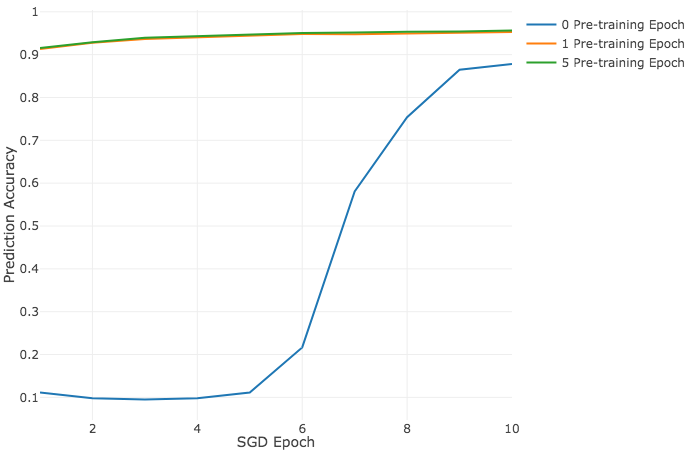
\includegraphics[scale=0.3]{images/iteration_two/pt/rbm_pretraining.png}
	\caption{SAE MSE By Scaling \newline The three series above show the classification accuracy scores (percentage) by epoch on an AutoEncoder which was used to classify MNIST images. The series were trained with 0, 1 and 5 pre-training epochs, and show a clear improvment in having an epoch of pre-training in the SAE formation (though not much for more than 1).}
	\label{figure-pretraining-effect}
	\end{figure}		
		
	Having considered the implementation to be correct and effective in the classic use case, it was then trialled on the following SAE configuration, with the results in the graphs below.
	\begin{itemize}
		\item Data: Closing prices for AGL \& ACL
		\item Processing: Time windows of 1, 5 and 20 (thus an input vector of size 6)
		\item Encoding Layer Activations: Sigmoid and Linear
		\item Encoding Layer Size: 5
		\item Hidden Layer Size: 15
		\item Number of Hidden Layers: 1, 2
		\item Learning Rates: 0.0000001, 0.00001, 0.001, 0.1, 1.0, 2.0
	\end{itemize}
		
	\begin{figure}[H]
	\centering 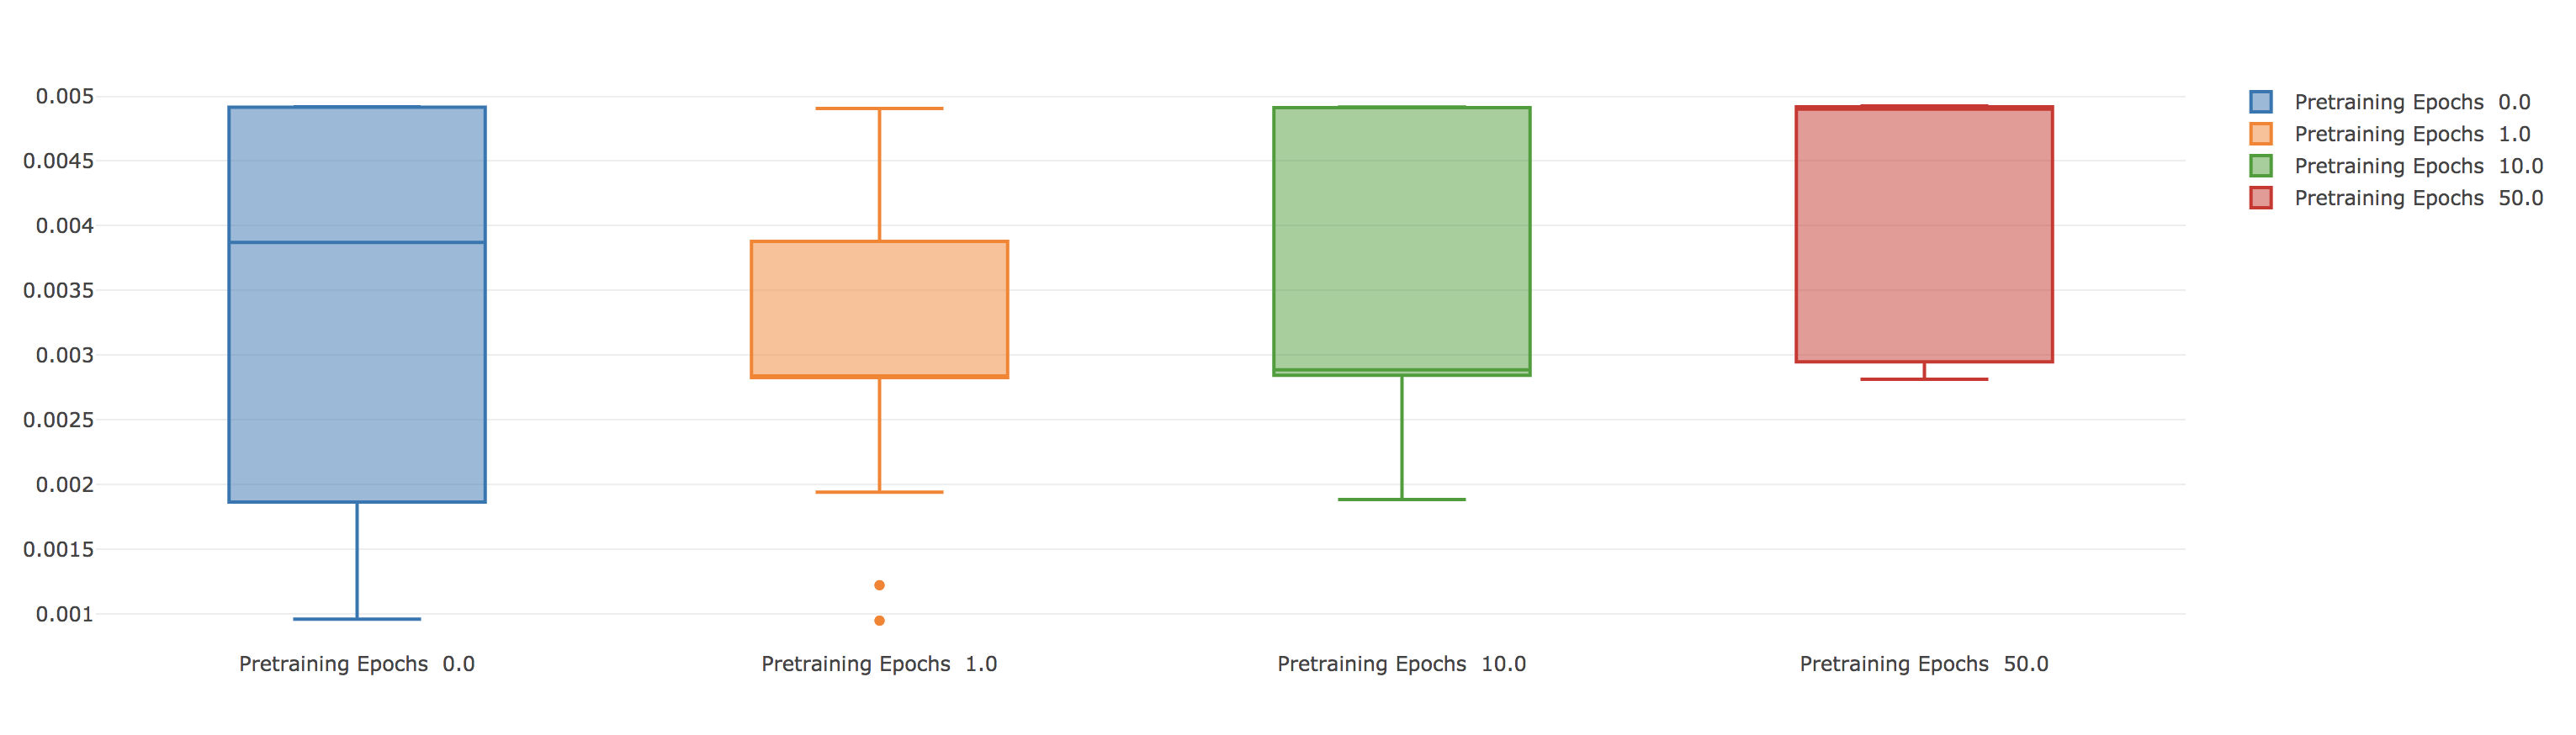
\includegraphics[scale=0.3]{images/iteration_two/pt/SAE_Pre-training_epochs_Min_Test_MSE.png}
	\caption{Pre-training Effects on financial SAE \newline The boxplots here show the summary of configuration performances, by minimum MSE achieved, grouped according to the number of pre-training epochs which the network had. There is a clear favour to having no pre-training in this scenario.}
	\label{figure-it2-pretraining-effect}
	\end{figure}		

	\begin{figure}[H]
	\centering 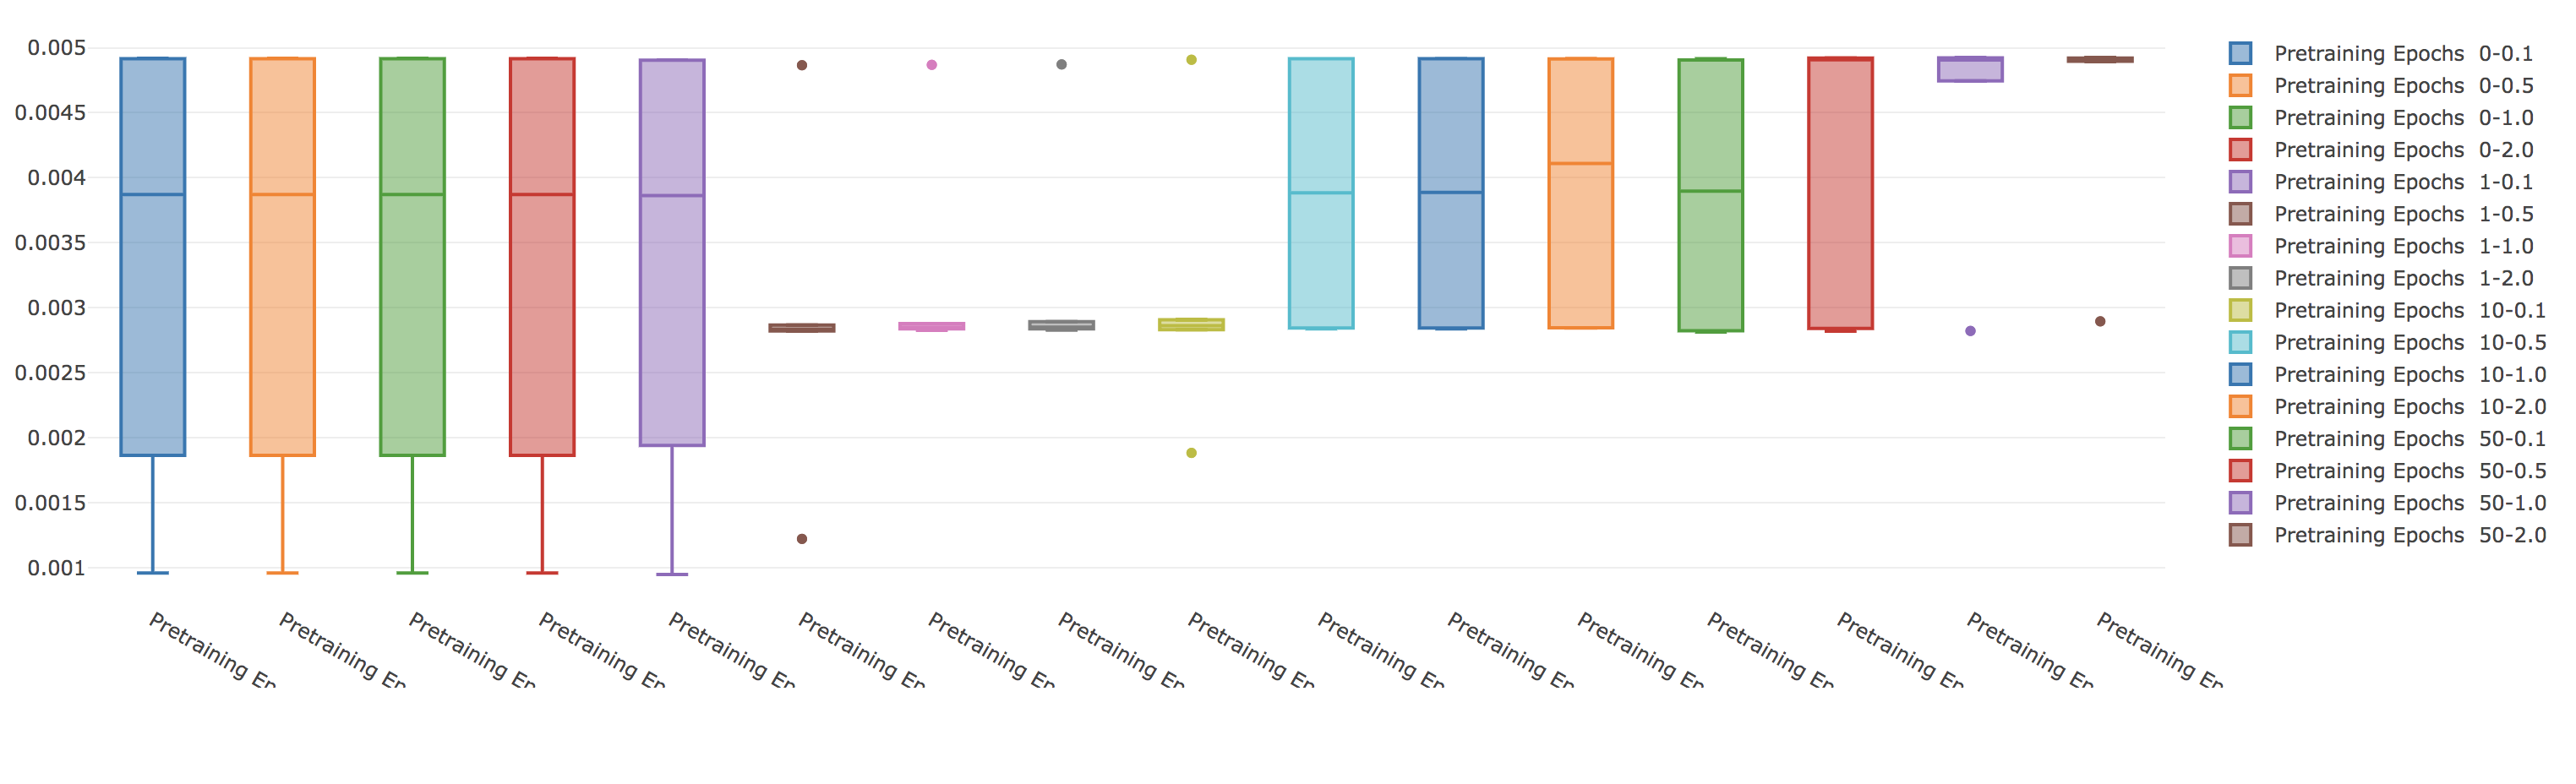
\includegraphics[scale=0.3]{images/iteration_two/pt/SAE_Pre-training_Learning_Rates_epochs_Min_Test_MSE.png}
	\caption{Pre-training Effects on financial SAE, by learning rate \newline These boxplots show the same as above, but further grouped by learning rate. We can see the few samples that appears to be benefiting from having 1 epoch of pre-training are simply a result of the learning rate being small enough so as not to have much effect.}
	\label{figure-it2-pretraining-effect2}
	\end{figure}		
		
		
		
		
	\paragraph{SAE Linear Activation Tests}		
	
	In consideration of the previous iterations results, numerous tests were run to assess the efficacy of Linear Activations in the encoding and output layers of the SAE networks. The list of configuration combinations are below.
	\begin{itemize}
		\item Data: Closing Prices for ACL, AGL, AMS, AOD, BAW, BIL, BVT, CFR, CRH, DDT
		\item Data Windows: 1, 5, 20 (thus input of 30)
		\item Data Scaling: Normalize, Standardize
		\item Weight Init,: Xavier Glorot Uniform
		\item All Layer Encodings: Sigmoid, ReLU, Linear (split by hidden, encoding and output)
		\item Encoding Layer Size: 5, 15, 25
		\item Hidden Layer Size: 60, 120
		\item Number of Hidden Layers: 1, 2, 3
		\item Learning Rates: Various for each different activation type (chosen by hidden activation used)
	\end{itemize}
		
	\begin{figure}[H]
	\centering 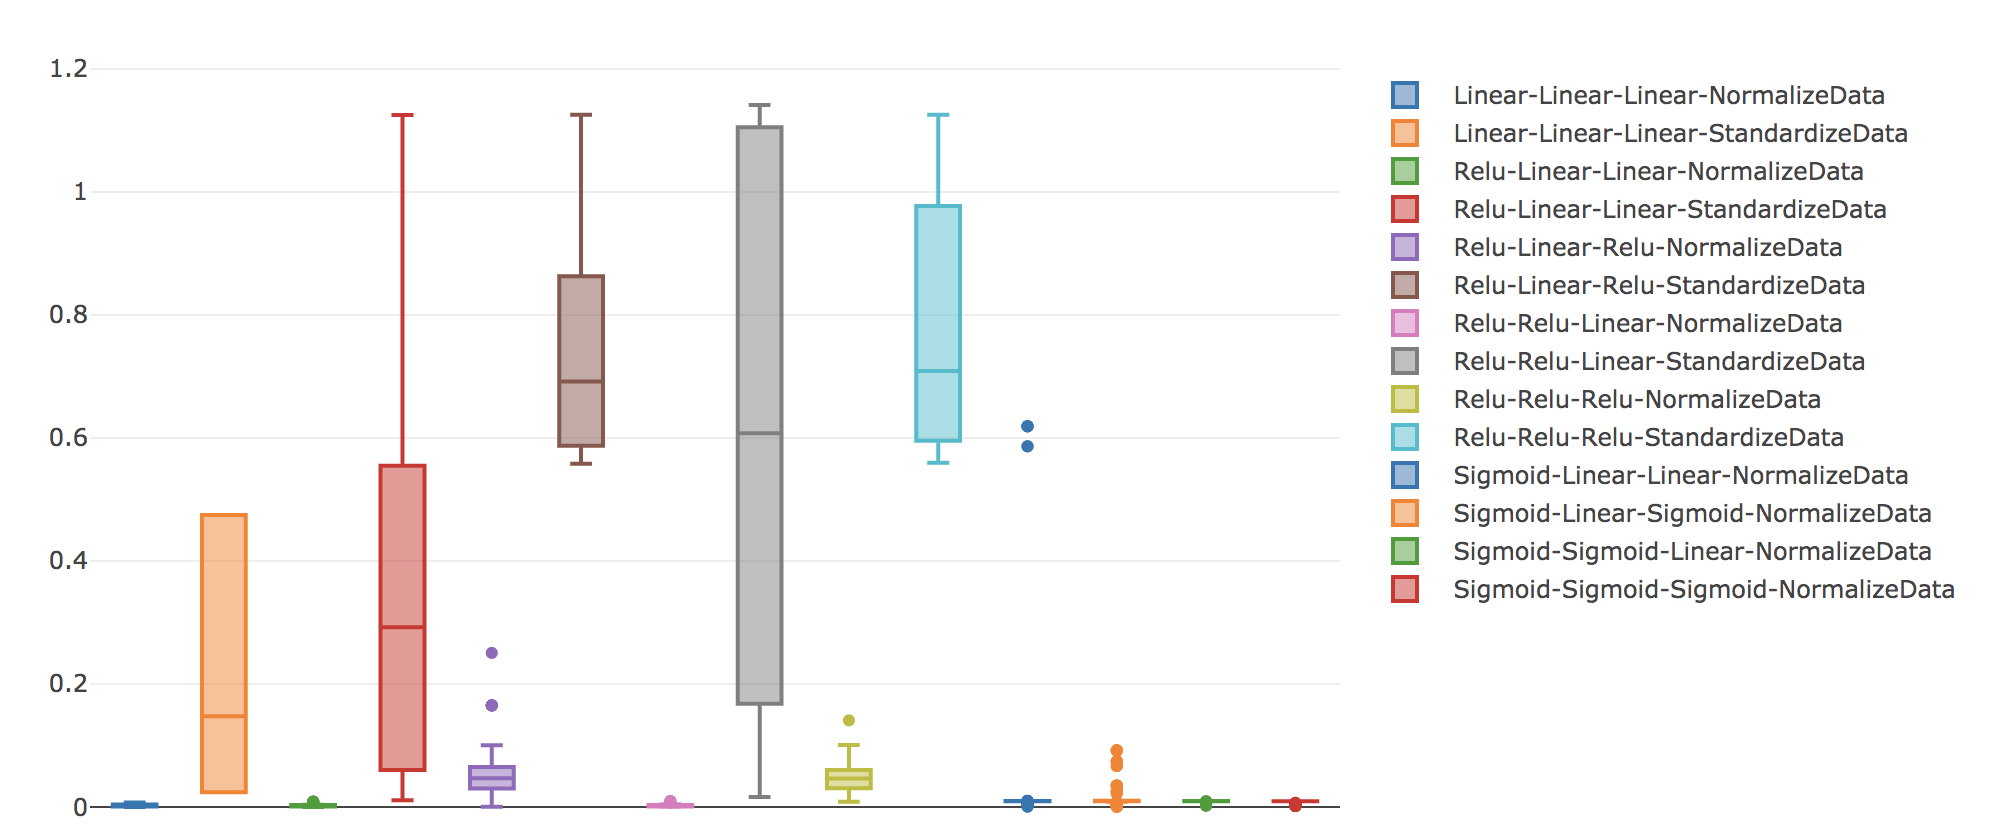
\includegraphics[scale=0.3]{images/iteration_two/linear/0Scaling_and_Activation_Combos_Min_MSE.png}
	\caption{Effects of Standardizing \& ReLU Output \newline These boxplots show the MSE scores for the combinations run grouped by 'Hidden Activation-Encoding Activation-Output Activation-Scaling Technique. There is significantly poorer performance when Standardizing is used instead of Normalizing or when there is a ReLU output activation. These configurations are excluded from the graphs below.}
	\label{figure-it2-scaling-and-relu}
	\end{figure}				
		
	\begin{figure}[H]
	\centering 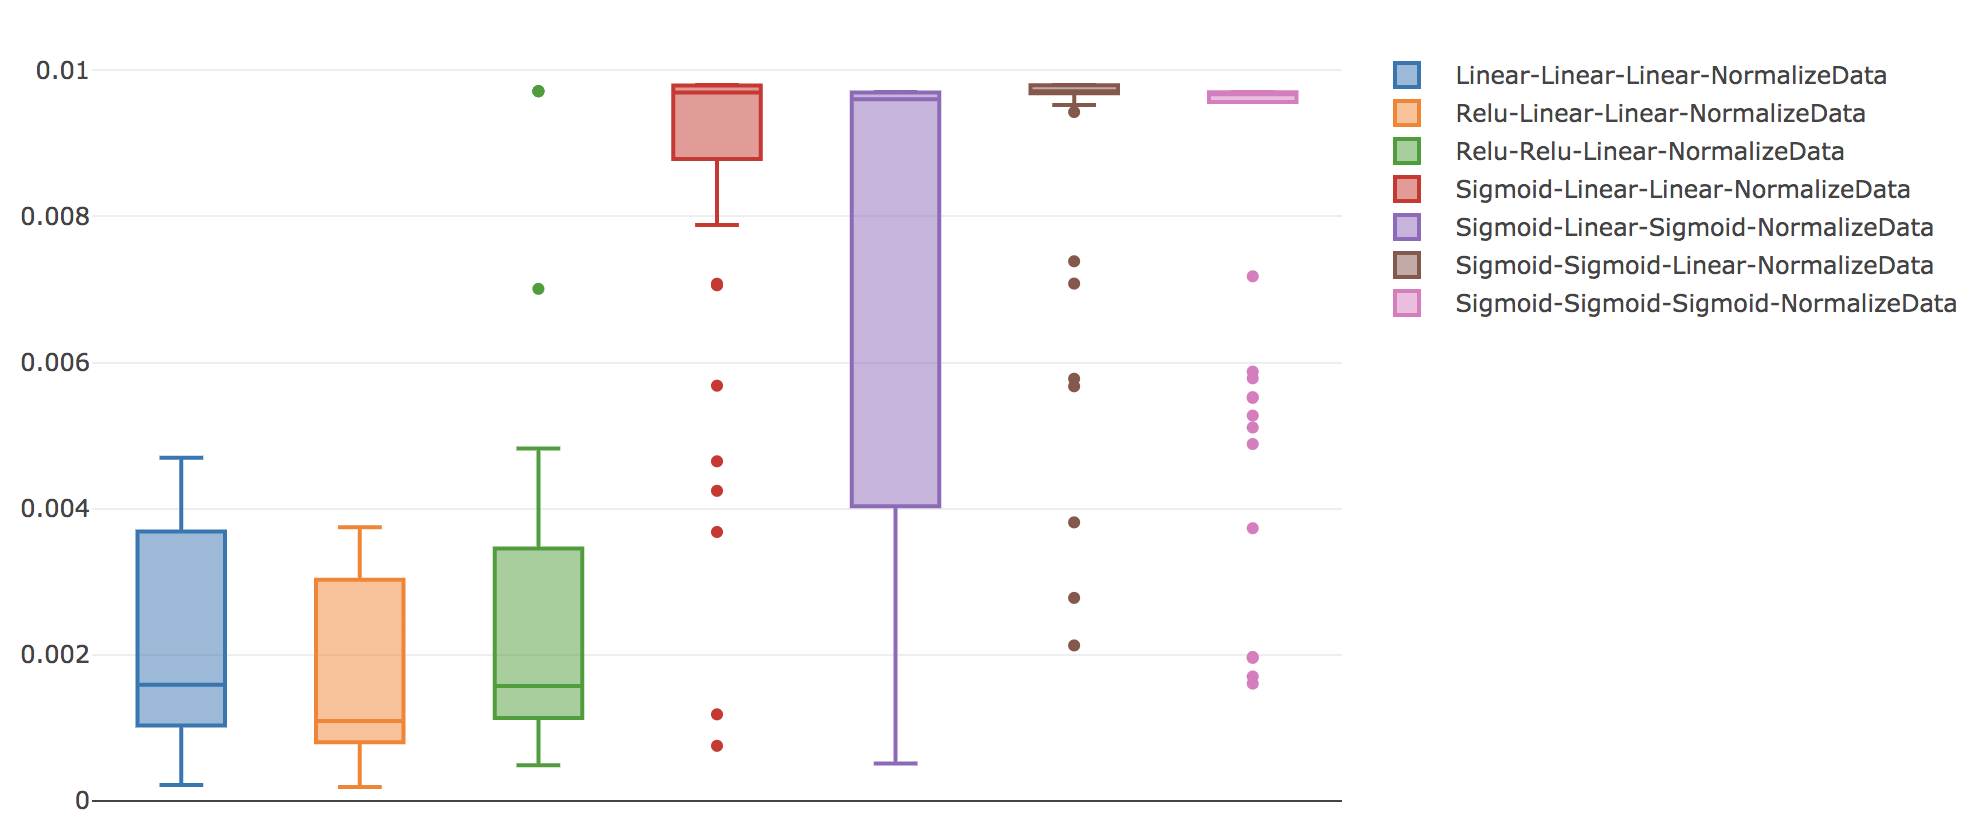
\includegraphics[scale=0.3]{images/iteration_two/linear/1Activation_Combos-Min_MSE.png}
	\caption{Effects of Linear Activation \newline This is the same data as in Figure 4, focusing on the more effective configurations. We can see Sigmoid has largely poor performance unless there is a Linear encoding layer (a widely experienced behaviour), and seems mostly unable to outperform a fully linear network. The best configuration is Relu Hidden layers, with Linear encoding and Output - this makes sense with the non-linear benefit at hidden layers but with less loss of error signal and information at the output and encoding layers.}
	\label{figure-it2-linear-act}
	\end{figure}				
		
	\begin{figure}[H]
	\centering 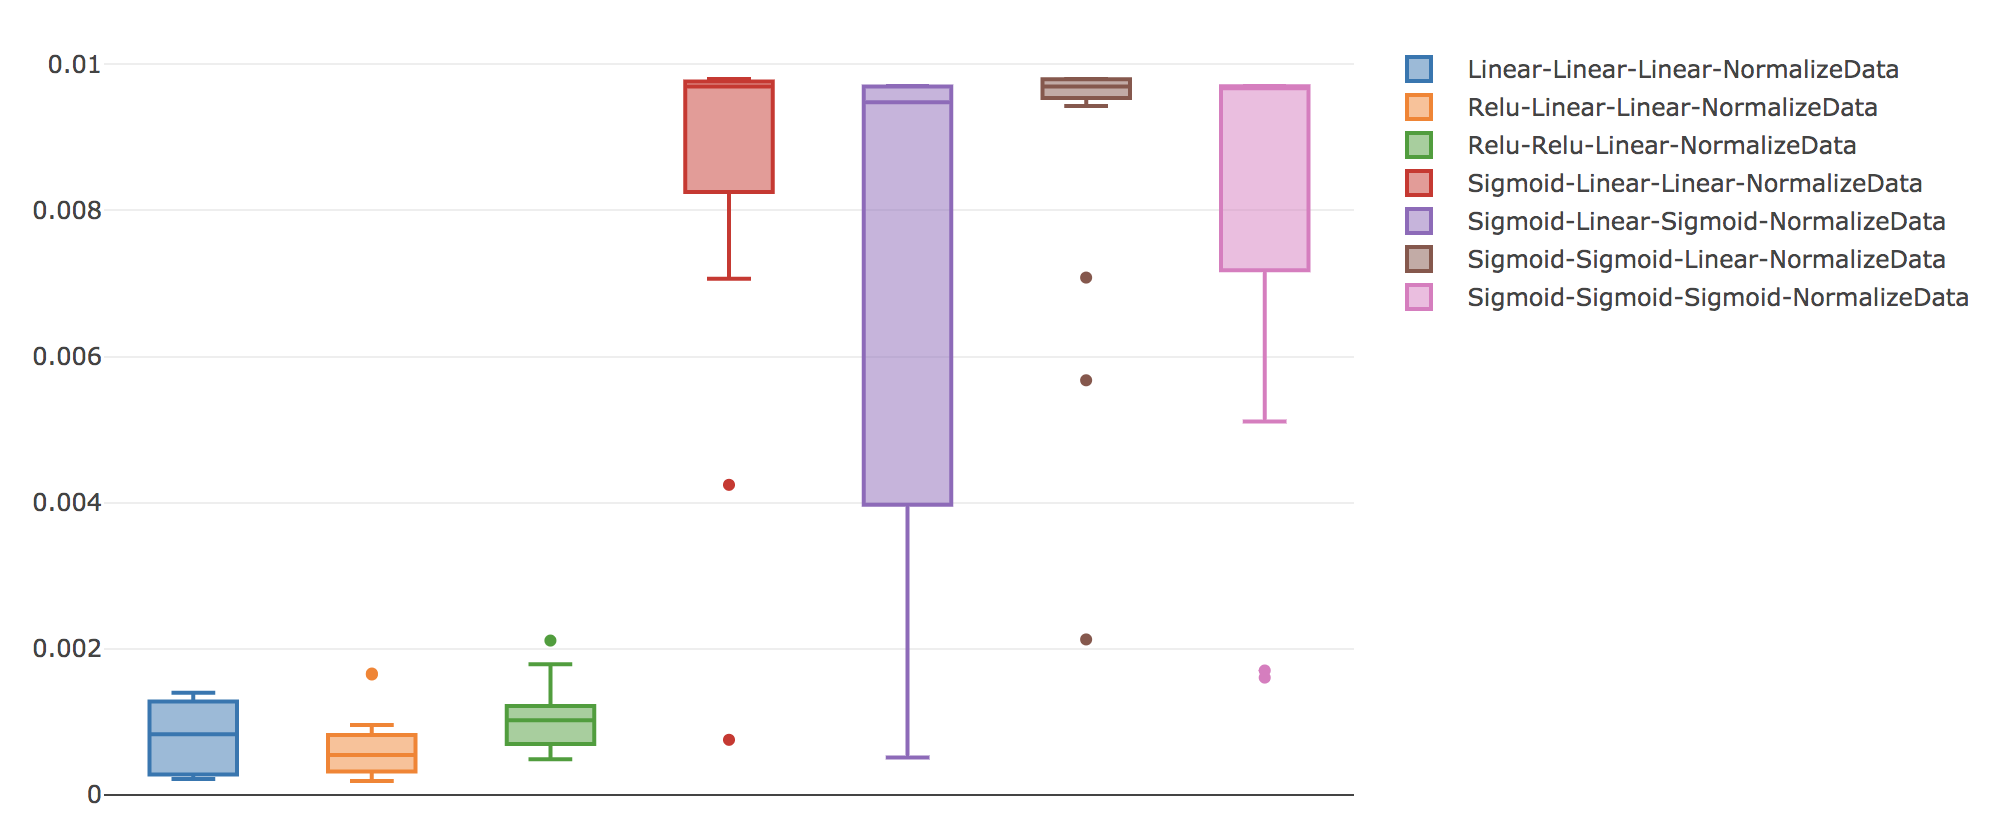
\includegraphics[scale=0.3]{images/iteration_two/linear/3Encoding_25_Activation_Combos_Min_MSE.png}
	\caption{Encoding Size 25 \newline These plots show the performance for all configurations with an encoding layer size of 25 (input 30). There is once again a surprisingly high performance in the fully linear network.}
	\label{figure-it2-encoding25}
	\end{figure}				

	\begin{figure}[H]
	\centering 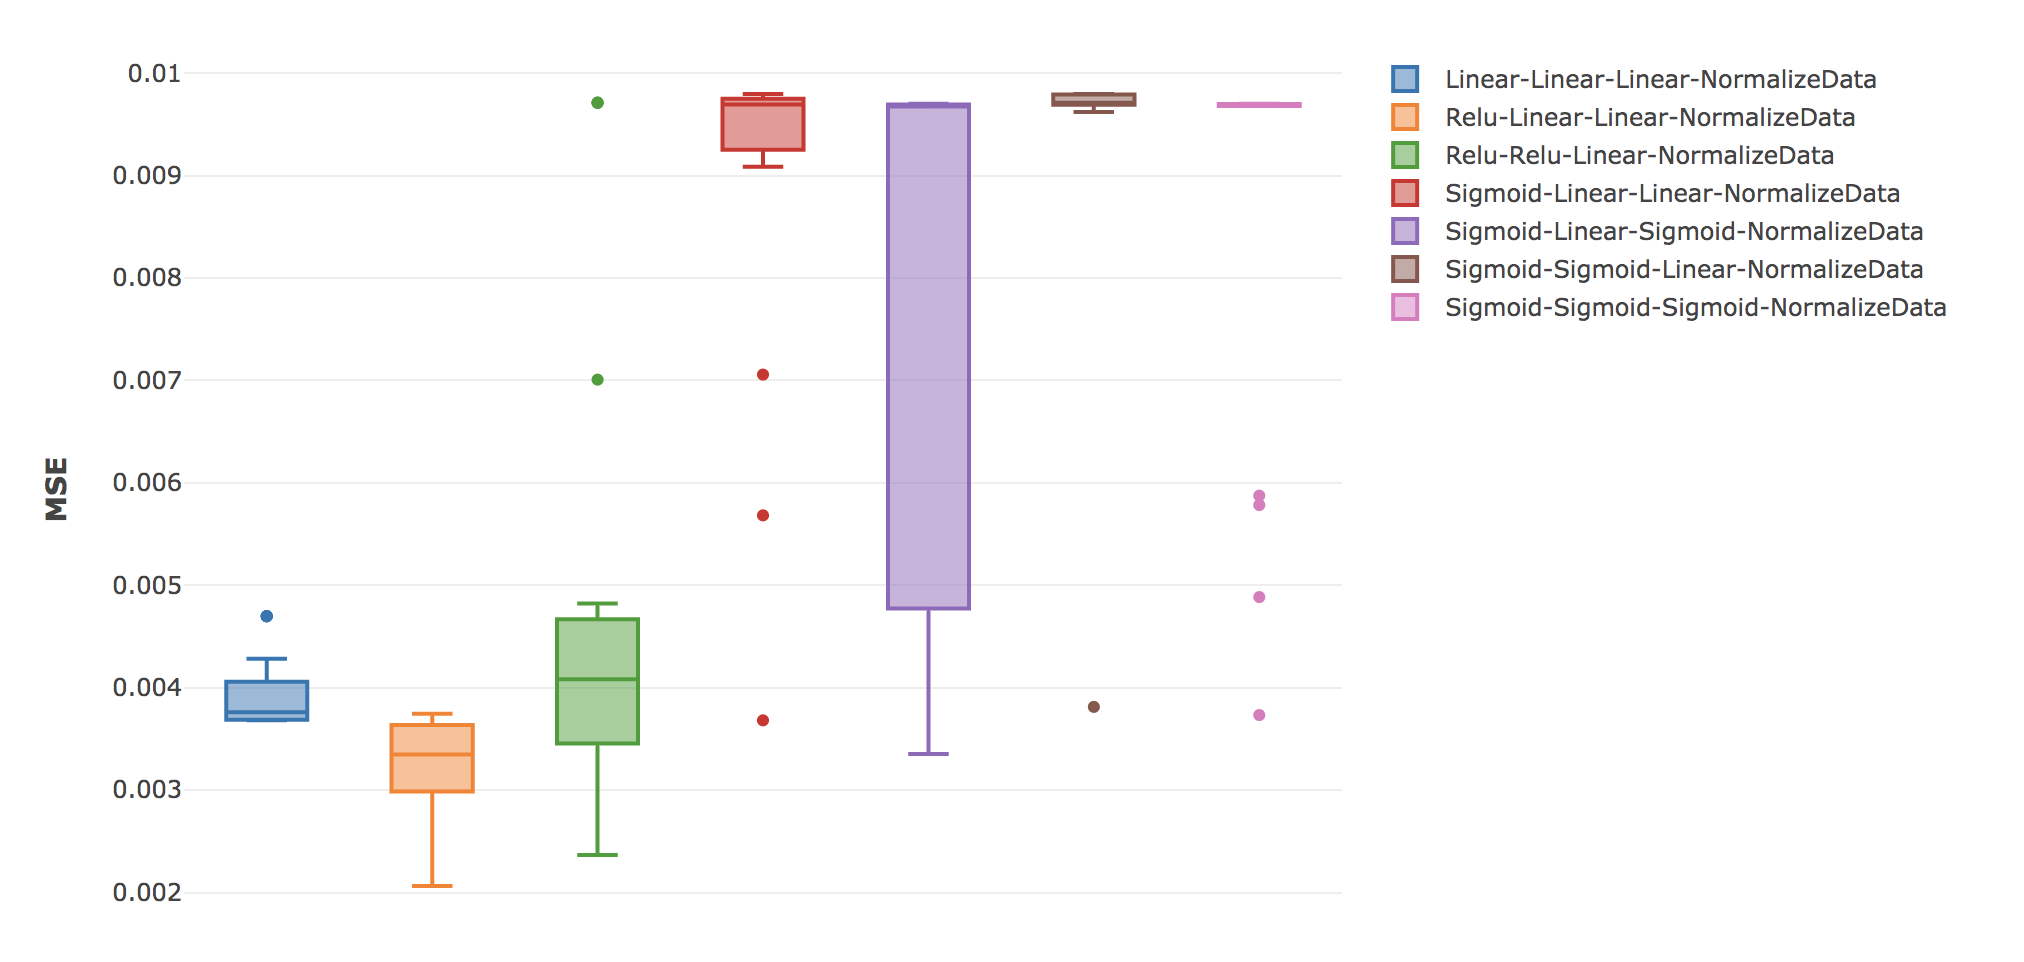
\includegraphics[scale=0.3]{images/iteration_two/linear/4Encoding_5_Activation_Combos_Min_MSE.png}
	\caption{Encoding Size 5 \newline These plots show the performance for all configurations with an encoding layer size of 5 (input 30). Here we finally see the benefit of non-linear activations in the ReLU based newtorks, which the fully linear is not able to outperform.}
	\label{figure-it2-encoding5}
	\end{figure}				
		
	\begin{figure}[H]
	\centering 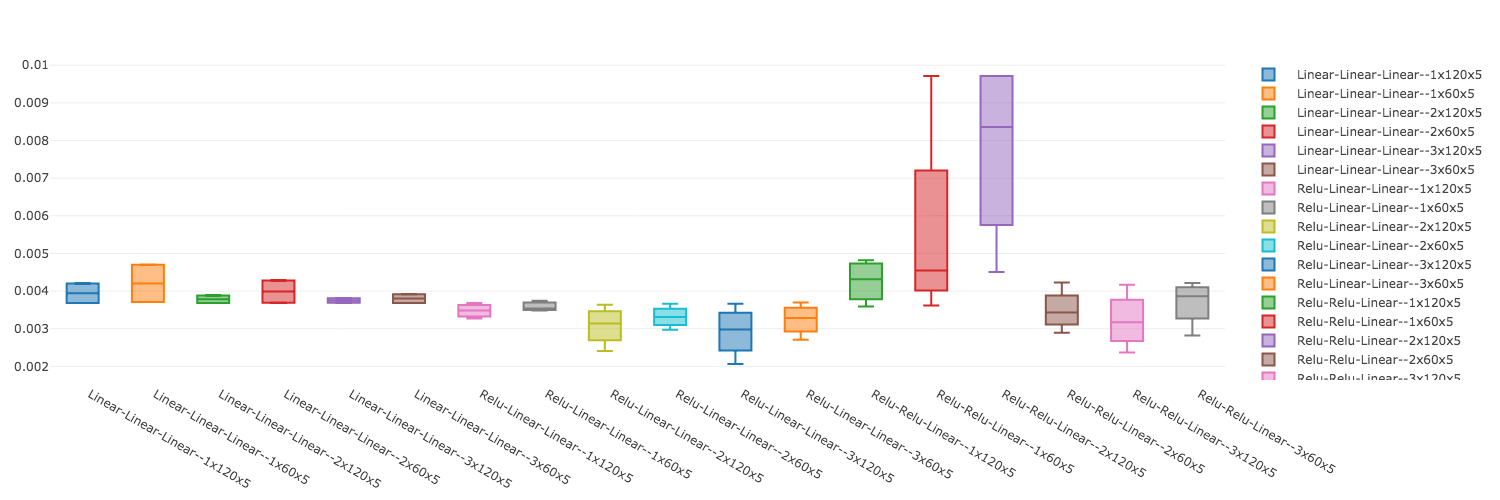
\includegraphics[scale=0.3]{images/iteration_two/linear/5Network_Size_Activation_Combos_for_Encoding_5_Min_MSE.png}
	\caption{Performance by Network Size 
		\newline We can further break these down by network size, and see performance is as one would hope, with the best ReLU configurations corresponding with more layers and of larger sizes.}
	\label{figure-it2-networksize-effect}
	\end{figure}				
		
		
	\paragraph{Denoising SAEs}
	
	Using the same data and general set up as above, a series of tests were run for DSAE using the best ReLU configurations and a gaussian noise process such that $\tilde{x} = \mathcal{N}(x, \sigma) $
		
	\begin{figure}[H]
	\centering 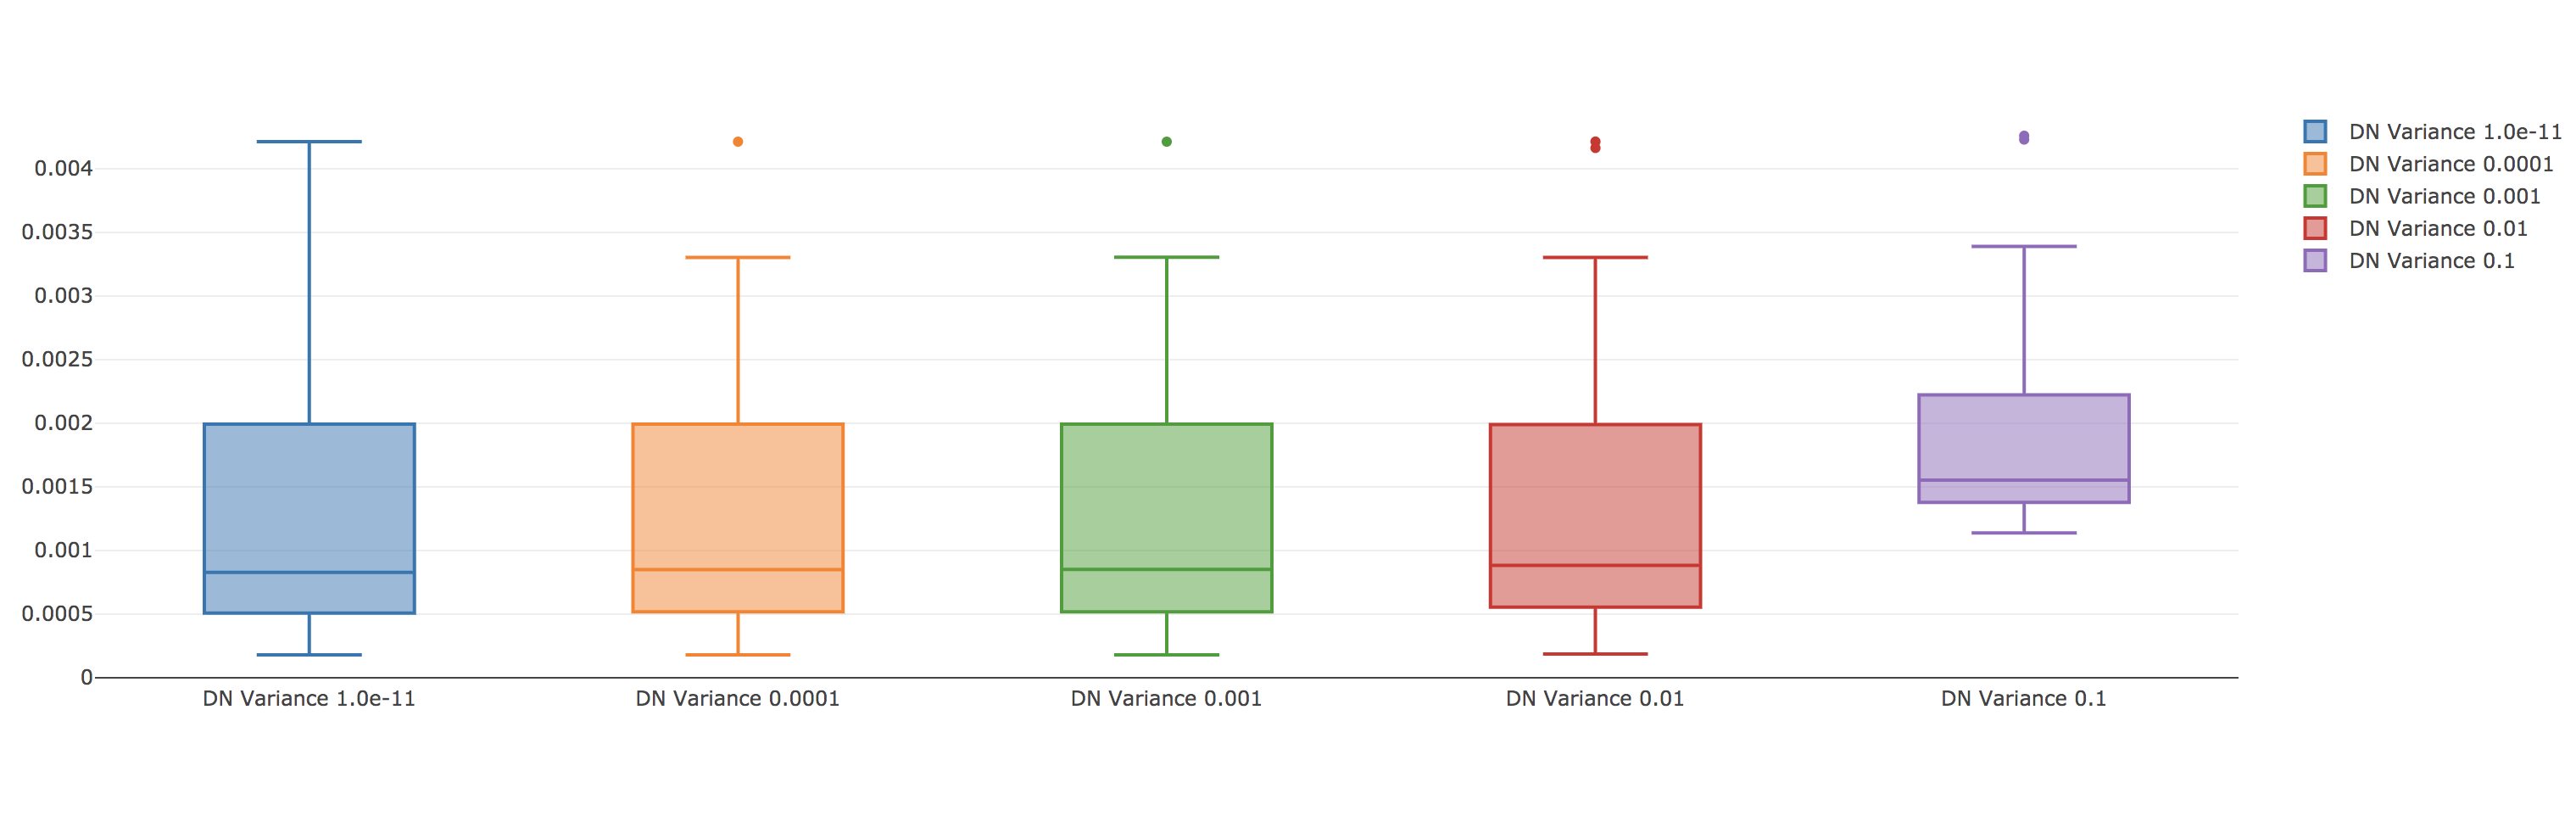
\includegraphics[scale=0.3]{images/iteration_two/denoise/denoising.png}
	\caption{Performance by Denoising Variation
		\newline The above groupings show the decreasing SAE performance as the level of denoising is increased. The grouping with variance 1.0e-11 essentially represents no denoising.}
	\label{figure-it2-denoise}
	\end{figure}						
		
		
	\paragraph{Linear Activations in FFN}
	
	A series of predictive FFN networks were run, with the following combinations
	
	\begin{itemize}
		\item SAEs: Best performance (lowest MSE) of encoding sizes 3, 6, 9, 12, 15 (input 18), of both Limited Scaling and typical Scaling methods
		\item Output Activations: ReLU, Linear
		\item Hidden Activations: ReLU, Linear
		\item Layer Sizes: 40, 80
		\item Number of Layers: 1, 3
		\item Various Learning rates for SGD \& OGD training
	\end{itemize}
		
		\begin{figure}[H]
			\centering 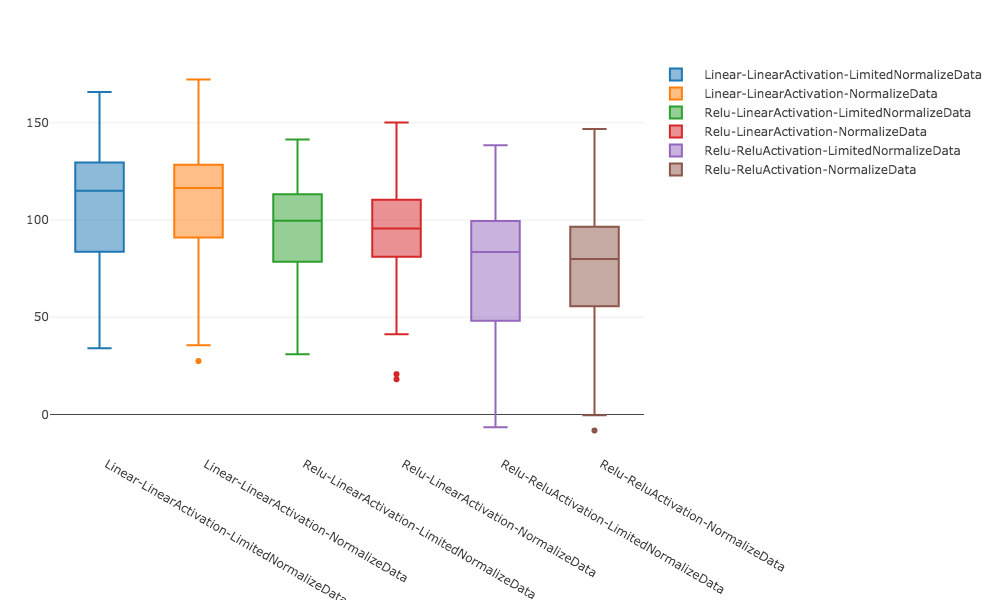
\includegraphics[scale=0.3]{images/iteration_two/linear-ffn/Scaling_Methodolgy_Profits.png}
			\caption{Linear Activations in FFN 
				\newline The above groupings show the profits generated for different combinations of Hidden Activation - Output Activation - Scaling Method (which is for both SAE and FFN). There are several takeaways:
				\newline 1. Higher performance of Linear networks (may be down to network size and amount of input data)
				\newline 2. The limited scaling technique is having a noticeable impact on profits
				\newline 3. The decrease in performance with ReLU output persists
				}	
			\label{figure-it2-linear-ffn_activations}
		\end{figure}						
		
	\newpage\large\textbf{Iteration 1: 12th April}
	
	\paragraph{Scaling}
	
	Unfortunately a bug resulted in the predictive networks not having a linear activation layer implemented (despite the naming). Current results suggest the limited scaling approach is resulting in worse MSE scores for both SAE and OGD. The OGD profits are also looking potentially worse (a linear activation implementation would need to be tested though).
	
	\begin{figure}[H]
		\centering 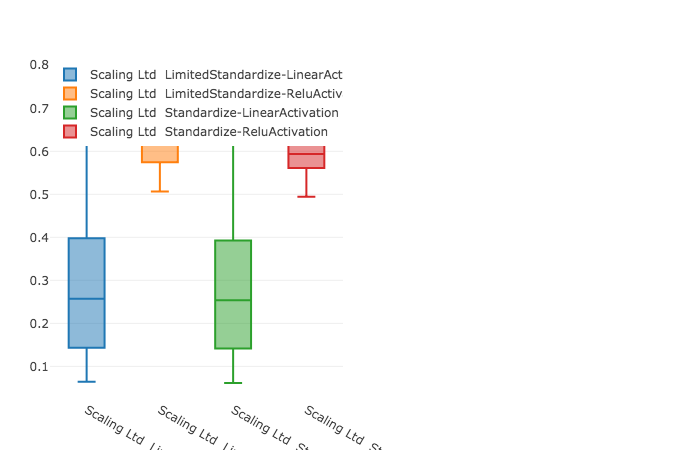
\includegraphics[scale=0.5]{images/iteration_one/sae_mse_by_scaling.png}
		\caption{SAE MSE By Scaling}
		\label{figure-synthetic-prices}
	\end{figure}

	\begin{figure}[H]
	\centering 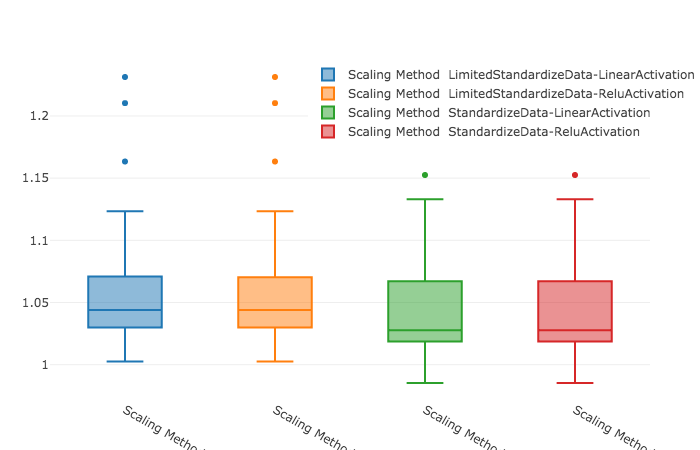
\includegraphics[scale=0.5]{images/iteration_one/ogd_mse_by_scaling.png}
	\caption{OGD MSE By Scaling}
	\label{figure-synthetic-prices}
	\end{figure}	

	\begin{figure}[H]
	\centering 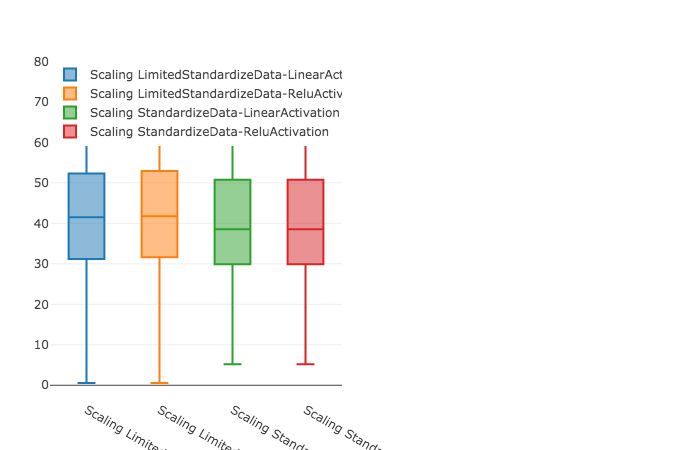
\includegraphics[scale=0.5]{images/iteration_one/ogd_profits_by_scaling.png}
	\caption{OGD Profits by Scaling}
	\label{figure-synthetic-prices}
	\end{figure}
	
	
	\paragraph{General Configurations \& CV}
	
	A larger set of configuration were run to test several concepts, as well as the removal of the CV step. The CV methodology needs to be kept for SAE in order to select a best set of SAEs, but is not strictly necessary for the SGD predictive training. In this case the trade off is that without CV a set number of epochs must be chosen (rather than monitoring the changes in OOS errors). All results below are run without CV in the SGD training.
	
	
	\begin{itemize}
		\item SAE Configurations:
		\begin{itemize}
			\item Encoding layers: 3, 6, 9, 12, 15 (input of 18)
			\item Layer sizes: 40x1, 40X2, 80X1, 80X2
			\item Various learning rates
			\item Different scaling functions \& output layers
		\end{itemize}
		\item FFN Configurations:
		\begin{itemize}
			\item Encoding Layers: 3, 9, 12
			\item Different scaling functions \& output layers  
			\item Various learning rates
			\item Layer sizes: 40x1, 40X2, 40x3, 80x1, 80x2, 80x3
		\end{itemize}
		\item Dataset Configurations:
		\begin{itemize}
			\item Synthetic Data
			\item 5000 timesteps
			\item Aggregation of 1, 7 and 30 to predict 2
			\item 60/40 split between SSGD and OGD
		\end{itemize}
	\end{itemize}

	The set of prices tested are shown below
	
	\begin{figure}[H]
		\centering 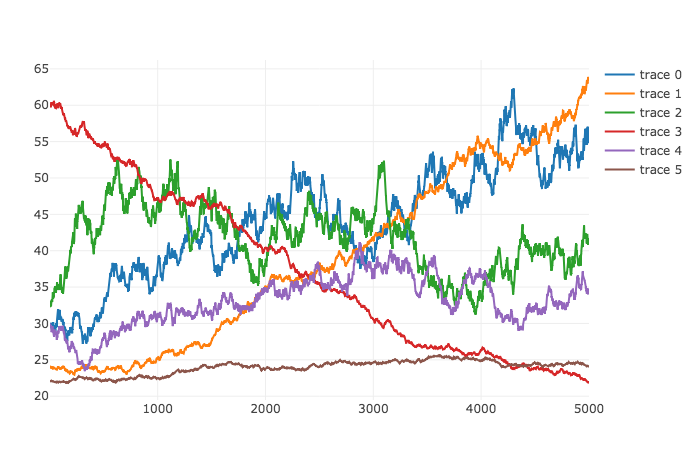
\includegraphics[scale=0.5]{images/iteration_one/price_plot.png}
		\caption{Price Plot}
		\label{figure-synthetic-prices}
	\end{figure}
	
	\begin{figure}[H]
		\centering 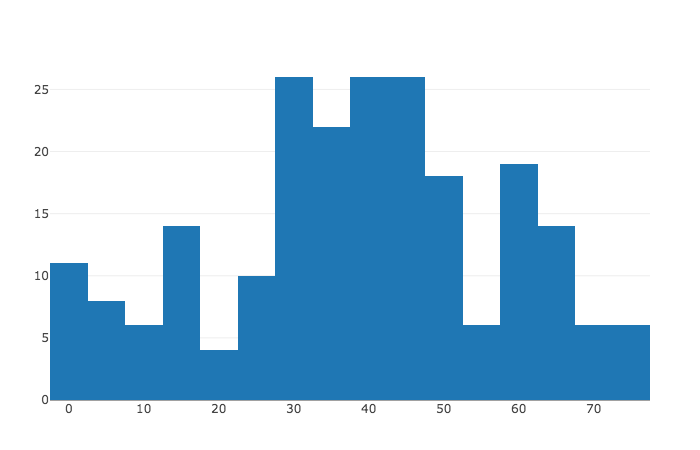
\includegraphics[scale=0.5]{images/iteration_one/profit_pdf.png}
		\caption{PDF of all Profits Generated}
		\label{figure-synthetic-prices}
	\end{figure}
	
	Profits by the SAEs chosen are below, suggesting that there is some level of feature selection being performed by the SAEs.
	
	\begin{figure}[H]
		\centering 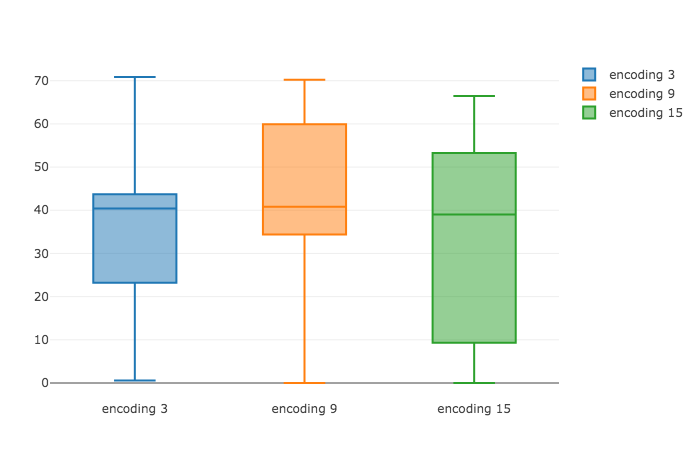
\includegraphics[scale=0.5]{images/iteration_one/profits_sae.png}
		\caption{SAE Profits}
		\label{figure-synthetic-prices}
	\end{figure}

	Profits by network structure are below, suggesting that simpler networks are performing better. This may point to some leve of overfitting occuring in the larger networks.

	\begin{figure}[H]
	\centering 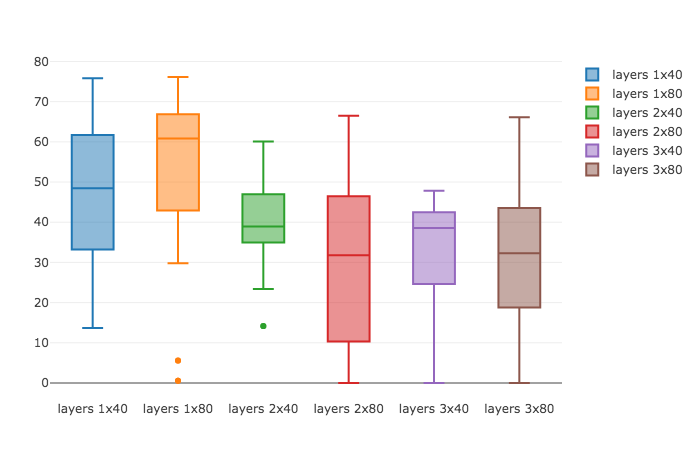
\includegraphics[scale=0.5]{images/iteration_one/profits_networks.png}
	\caption{Network Structure Profits}
	\label{figure-synthetic-prices}
	\end{figure}	
	
	
	\paragraph{Return Graphs}
	
	The graphs below show the cumulative return rates, profits and daily rates of the best network. The best network was chosen by MSE rather than profit, for reasons discussed below.
	
	\begin{figure}[H]
	\centering 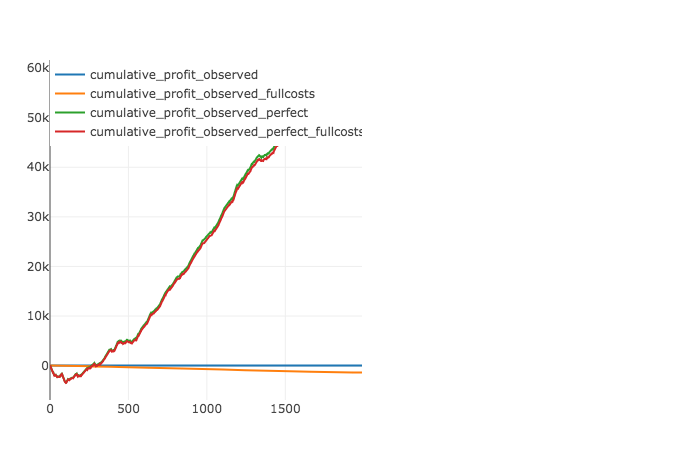
\includegraphics[scale=0.5]{images/iteration_one/results_cumulative_profits.png}
	\caption{Cumulative Profits}
	\label{figure-synthetic-prices}
	\end{figure}		
	
	\begin{figure}[H]
	\centering 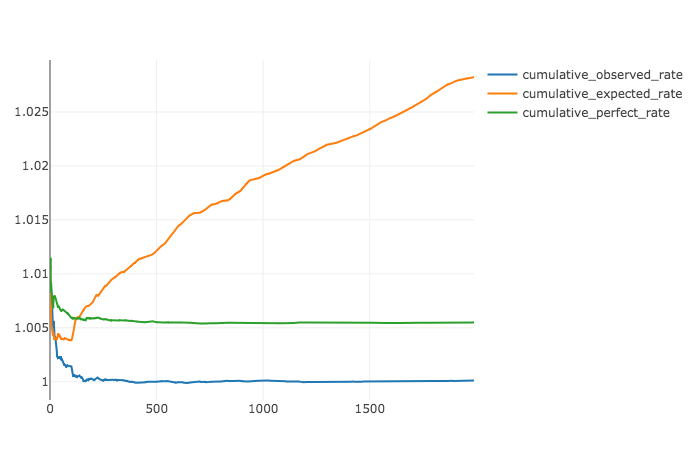
\includegraphics[scale=0.5]{images/iteration_one/results_cumulative_rates.png}
	\caption{Cumulative Return Rates}
	\label{figure-synthetic-prices}
	\end{figure}		
	
	\begin{figure}[H]
	\centering 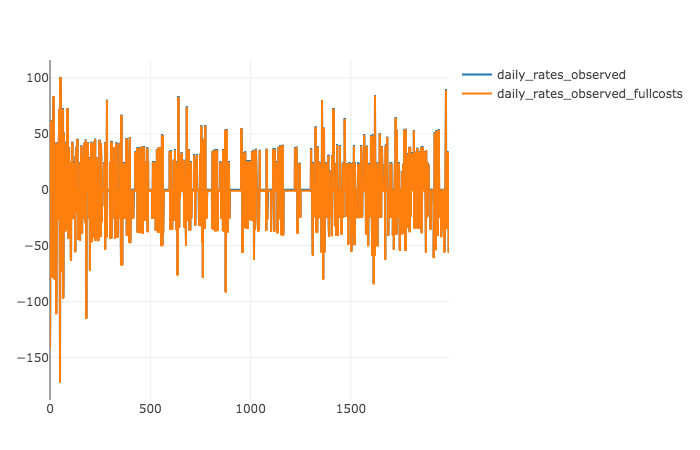
\includegraphics[scale=0.5]{images/iteration_one/results_daily_rates.png}
	\caption{Daily Rates}
	\label{figure-synthetic-prices}
	\end{figure}		
	
	
	\paragraph{Price Predictions}
	
	The price predictions are showing 2 problems: heaving oscillations occuring at most points, and the most profitable configuration having a relatively poor level of prediction.
	
	\begin{figure}[H]
		\centering 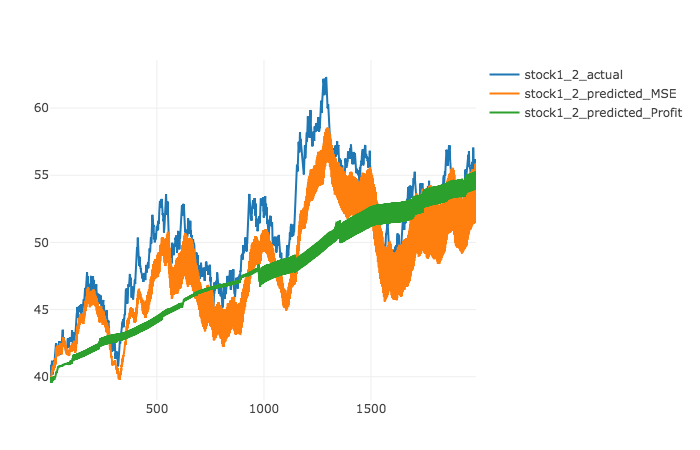
\includegraphics[scale=0.5]{images/iteration_one/stock1.png}
		\caption{Stock 1}
		\label{figure-synthetic-prices}
	\end{figure}		

	\begin{figure}[H]
	\centering 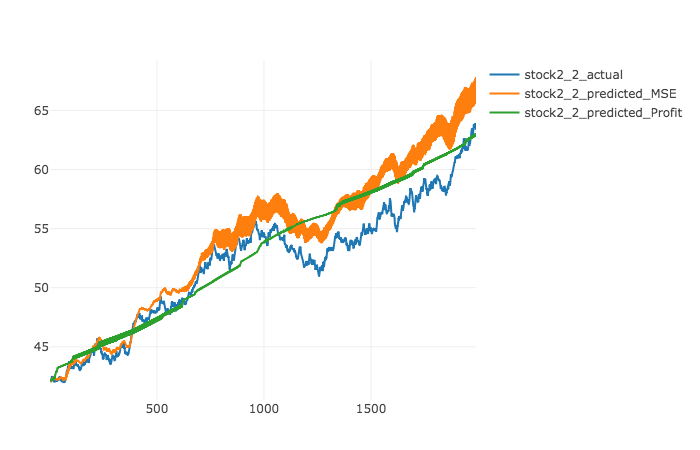
\includegraphics[scale=0.5]{images/iteration_one/stock2.png}
	\caption{Stock 2}
	\label{figure-synthetic-prices}
	\end{figure}		
	
	\begin{figure}[H]
	\centering 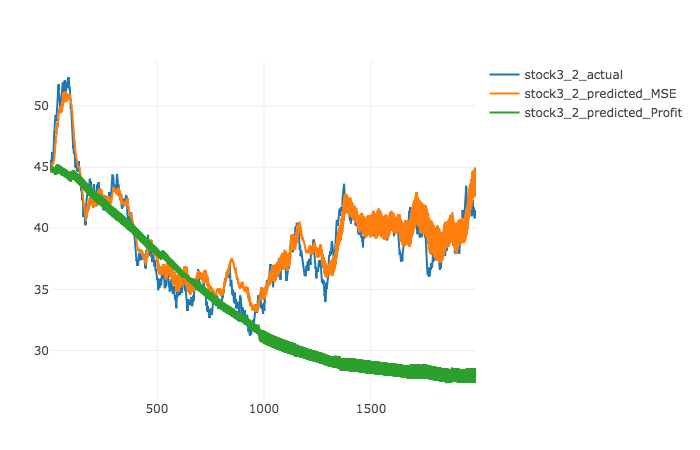
\includegraphics[scale=0.5]{images/iteration_one/stock3.png}
	\caption{Stock 3}
	\label{figure-synthetic-prices}
	\end{figure}		

	\begin{figure}[H]
	\centering 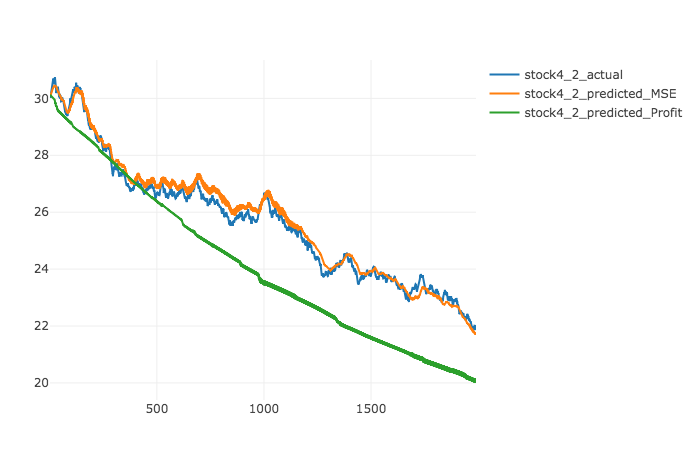
\includegraphics[scale=0.5]{images/iteration_one/stock4.png}
	\caption{Stock 4}
	\label{figure-synthetic-prices}
	\end{figure}		

	\begin{figure}[H]
	\centering 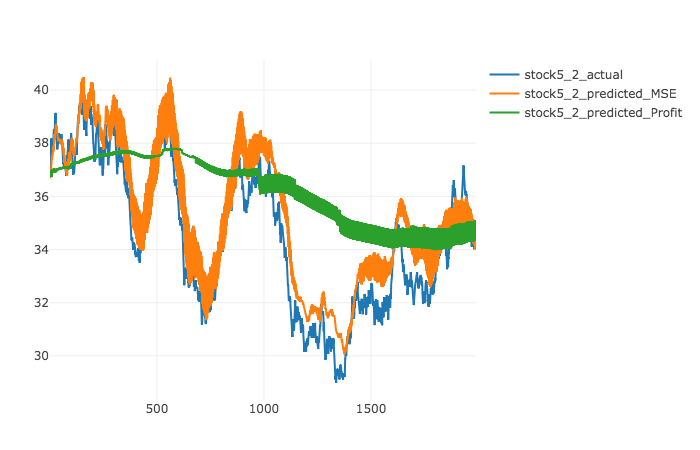
\includegraphics[scale=0.5]{images/iteration_one/stock5.png}
	\caption{Stock 5}
	\label{figure-synthetic-prices}
	\end{figure}		

	\begin{figure}[H]
	\centering 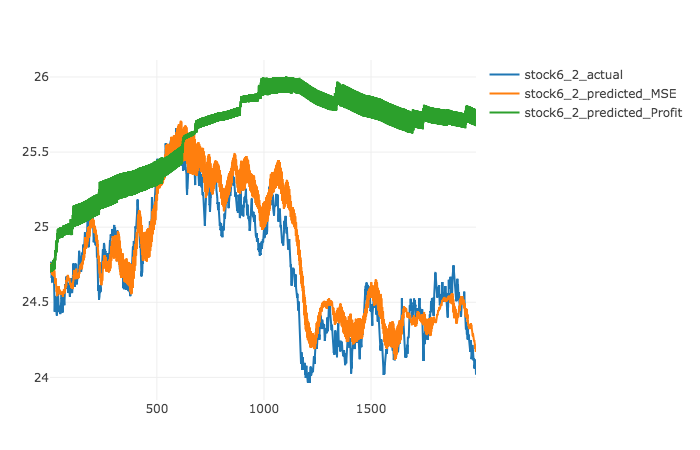
\includegraphics[scale=0.5]{images/iteration_one/stock6.png}
	\caption{Stock 6}
	\label{figure-synthetic-prices}
	\end{figure}		
	
	\paragraph{Sigmoid Pre-training}	
	
	The pre-training for weight initialization in the Sigmoid networks, which is supposed to improve performance, seems to be having an adverse effect:
	
	\begin{figure}[H]
		\centering 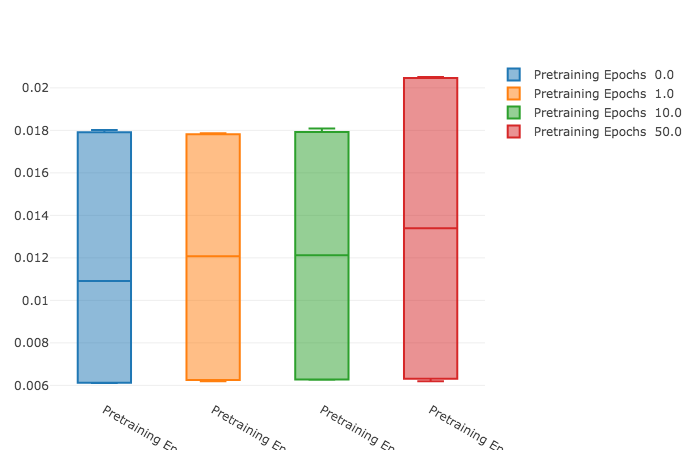
\includegraphics[scale=0.5]{images/iteration_one/pretraining.png}
		\caption{Stock 6}
		\label{Pre-training MSE performance}
	\end{figure}		
	
	
	\newpage
	
	
	
	
	
	
	
	
	
	\bigskip\large\textbf{4. Future Status and Next Iteration}\bigskip\normalsize
	
	The results of the current set highlight that overfitting is the biggest problem at the moment. A set of features, as noted below, will be implemented prior to proceeding with tests.
	
	\paragraph{Next Iteration}

	
	\paragraph{Critical Decisions and Points of Concern}

	\begin{itemize} 
		\item[$\bullet$] Scaling Choices
		\item[$\bullet$] Price Prediction oscillations		
		\item[$\bullet$] Effect of profit strategy on poor prediction models
		\item[$\bullet$] Pre-training efficacy		
		\item[$\bullet$] Decide on data splits and what should be used for CSCV - MinBTL method?
		\item[$\bullet$] Decide on data windows - aribtrary choices or.. ?
	\end{itemize}

	\paragraph{Non-Critical Features}

	\begin{itemize}
		\item[$\bullet$] Denoising SAEs
	\end{itemize}	

	\paragraph{Dissertation to-do list}

	\begin{itemize}
		\item Literature Review: There are various inclusions and ammendments to be made here (particularly around data windows \& varance initializations)
		\item Reformatting of Algorithms through document
		\item Papers and references to add: Wilcox \& Debbie Hierarchical Paper; Crutchfield \& Farmer: Geometry of Time Series; F Takens: Detecting strange attractors in turbulence; Reference Riaz
		\item General formatting changes necessary
		\item Various to-do notes throughout paper
	\end{itemize}	

	\newpage\bigskip\large\textbf{5. Milestones \& Deliverables}\normalsize
	
	

	\begin{table}[h]
		\begin{tcolorbox}[tabularx*={\arrayrulewidth0.6mm}{X||X},fontupper=\normalsize\sffamily,colback=white!10!white,colframe=black!40!]
			
			\centerline{\textbf{Finish Date}} &\centerline{\textbf{Item}} \\\hline
			\centerline {Requires Corrections} & {1 Literature Review}\\\hline
			\centerline {In Progress} & {2 Data Collection}  \\\hline
			\centerline {\cellcolor{gray!25}  Done}  & {\cellcolor{gray!25}  3 Data Log Fluctuation Processing}  \\\hline
			\centerline {\cellcolor{gray!25}  Done} & {\cellcolor{gray!25}  4 SAE Implementation}  \\\hline
			\centerline {\cellcolor{gray!25}  Done} & {\cellcolor{gray!25}  5 Online FFN/LSTM Implementation} \\\hline
			\centerline {\cellcolor{gray!25}  Done} & {\cellcolor{gray!25}  6 CSCV Implementation} \\\hline		
			\centerline {\cellcolor{gray!25}  Done} & {\cellcolor{gray!25}  7 Synthetic Data Generation} \\\hline					
			\centerline {\cellcolor{gray!25}  Done} & {\cellcolor{gray!25}  8 Finalise Implementation Process} \\\hline
			\centerline {\cellcolor{gray!25}  Done} & {\cellcolor{gray!25}  9 Database Implementation} \\\hline
			\centerline {\cellcolor{gray!25}  Done} & {\cellcolor{gray!25}10 Learning Optimizations} \\\hline			
			\centerline {} & {11 Test full implementation on synthetic data} \\\hline
			\vspace{0.1mm}  \centerline {} &\vspace{0.1mm}   {12 Test full implementation on actual dataset} \\\hline
			\vspace{0.1mm}  \centerline {} &\vspace{0.1mm}   {13 Statistical Analysis (incl. profitability of trading strategy)} \\\hline
			\vspace{0.1mm}  \centerline {} &\vspace{0.1mm}   {14 Write up \& Revisions} \\\hline
									
		\end{tcolorbox}
	\end{table}
	\FloatBarrier

	\newpage\bigskip\large\textbf{6. Process Implementation}\bigskip\normalsize

	The steps below indicate how everything is expected to fit together at a high level perspective:
	
	\begin{itemize}
		\item [1] Data preparation
		\begin{itemize}
			\item[$\bullet$] The data is processed into day to day log fluctuations
			\item[$\bullet$] At each time point, rolling historic summations are calculated (e.g. the past 1, 7 and 30 days)
			\item[$\bullet$] At each time point, rolling future summations are calculated (e.g. the next 2 days)
		\end{itemize}
		\item [2] Data Segregation
		\begin{itemize}
			\item[$\bullet$] The processed dataset is split into 2 parts, to be used for the following processes: SAE/SGD training and OGD training (e.g. 60\%, 40\%)
			\item[$\bullet$] Bailey's MinBTL method should be considered to determine this split length
		\end{itemize}	
		\item [3] SAE Training
		\begin{itemize}
			\item[$\bullet$] The dataset defined for SAE/SGD is used to train the auto-encoder networks (using either RBM pretraining/weight initialization algorithms + SGD)
			\item[$\bullet$] Notably, this SAE/SGD dataset will itself be split into training \& testing portions in order to train and validate the SAE network
			\item[$\bullet$] The SAE training does not suffer from the same backtesting concerns as for the predictive network. A full set of models for difference encoding layers can be trained to sufficient performance, and then used as a configuration aspect for the predictive training.
		\end{itemize}		
		\item [4] FFN/SGD Training
		\begin{itemize}
			\item[$\bullet$] The same SAE/SGD portion of the data will then be used to train the FFN network to predict future prices, using the implemented SGD algorithm \& optimizations.
		\end{itemize}			
		\item [5] OGD Training
		\begin{itemize}
			\item[$\bullet$] The second portion of data will be used to train and optimize the FNN from 4 for OGD. The purpose of this will be to optimize to train the network and produce returns.	
		\end{itemize}			
		\item [6] Returns generations
		\begin{itemize}
			\item[$\bullet$] A basic trading strategy will be used to generate returns from the predicted and actual prices in the holdout dataset. These returns for each time period and each configuration of the model defined by steps 3-5 will form the M matrix for the CSCV process.
		\end{itemize}	
		\item [7] CSCV \& PBO
		\begin{itemize}
			\item[$\bullet$] Using the M matrix from 6, the CSCV process will be run which will then allow a calculation of PBO.
		\end{itemize}		
	\end{itemize}

	\newpage\bigskip\large\textbf{7. Meeting Minutes}\bigskip\normalsize	
	\paragraph{16th June 2018}
	\begin{itemize}
		\item[$\bullet$] Literature Review
		Include: Wilcox \& Debbie Hierarchical Paper; Crutchfield \& Farmer: Geometry of Time Series; F Takens: Detecting strange attractors in turbulence; Reference Riaz
		\item[$\bullet$] Implementation
		\begin{itemize}
			\item[$\bullet$] Key implementation point was the data segmentation choices
			\item[$\bullet$] LSTM network would resolve this point for us (CNN convolution could also potentially
			work)
			\item[$\bullet$] Non LSTM will run risk of correlating times with stocks
			\item[$\bullet$] Representation needs a mixture of time scales as well as the features
			\item[$\bullet$] Will be considering data for the entire index at any time point t
			\item[$\bullet$] Will need to consider how to address the changing constituents
			\item[$\bullet$] Aspect of how often the feature selection is updated (e.g. SDAE in online model)
			\item[$\bullet$] Does it get updated in the online model ?
			\item[$\bullet$] SDAE result should be similar to edge detection which will give set of predictions essentially
			\item[$\bullet$] Use known test cases for CSCV method development
		\end{itemize}
		\item[$\bullet$] Data
		\begin{itemize}
			\item[$\bullet$] Use simple noise with Gaussian distribution \& long trends to develop network models (6
			variations of increasing, decreasing and flat with low or high variability)
			\item[$\bullet$] Build backdated tests module with surrogate data afterwards
			\item[$\bullet$] Not going to try intraday data due to different nature of problem
			\item[$\bullet$] Implementation of either a flat file or MongoDB
			\item[$\bullet$] Important to include Volume datav
			\item[$\bullet$] Volume time -> might be far more predictable; volume and variance linked
		\end{itemize}
		\item[$\bullet$] Other
		\begin{itemize}
		\item[$\bullet$] Admin:Single document - table of contents (nice to have) with authors; sections etc. ; full doc with
		versioning; PDF + latex (always send both)
		\item[$\bullet$] 	Further Correspondence:
		* Iterate over FFN/LSTM implementations rather than starting with LSTM
		* For the meantime, assume the models do not differ fundamentally enough to be considered as
		separate for the PBO calculations
		\end{itemize}
	\end{itemize}		

	\paragraph{29th March 2019}
	
	\begin{itemize}
		\item Dissertation
		\begin{itemize}
			\item Generally frame the idea as a simplest high complexity framework in rational testing framework
			\item Need to highlight and sell the SAE separation in terms of reasoning and value
			\item SAE training updates: just make comment that not updating 
			\item Include discussion around decoupling of model components
		\end{itemize}
	
		\item Data Considerations
		\begin{itemize}
			\item 80/20\% split for SGD: Should this be used? May not be necessary in full process. Could also consider using all the data for OGD rather than SGD/OGD split.
			\item Split for SAE\&SGD/OGD split: Baileys MinBTL should at least be discussed, and possibly used.
			\item Prediction goal
			\begin{itemize}
				\item [1]: A 3/5 days average at end. Buy / sell according to above / below.
				\item [2]: 1-30 days distribution with error variances at each point. Consider how far ahead highest possible forecast is and what the spread on that is.—> outside scope but need to address to show it’s been thought carefully about Money management strategy for model (out of scope) but should have some consideration in terms of such a distribution
			\end{itemize}
		
			\item Scaling
			\begin{itemize}
				\item Paragraph or 2 showing this is a technical problem, and point out that want this learning to be ind. of normalisation 
				\item Currently choosing to normalise correctly in training set  
				\item Mention iterative normalisation which will converge: Can benchmark large covariance matrix against noise model for matrix and use PCA and plot eigen values for noise distribution. Would still be removing some level of signal -> and signal chosen should be as far outside noise model as possible.
			\end{itemize}
		
			\item Datasets
			\begin{itemize}
				\item Continue to use surrogate data for testing, and then use close \& intraday sets for actual results
				\item Daily data have enough to submit 
				\item Intraday: trade every 5 minutes? 
				\item Intraday will make a good inclusion and extension
			\end{itemize}
		\end{itemize}
	
		\item Results Reporting
		\begin{itemize}
			\item Nyquest frequency and breakdown on aliasing: need to discuss this to validate the [2] choice, and note that naive prediction could expose us to aliasing and fitting to the band ripple rather than underlying signal in prices
			\item Continue with and clearly state how the arithmetic money management strategy is working 
			\item Processing signals but generating P\&L based on the MMS
			\item The performance measure is based on these P\&L returns
			\item Generate daily P\&L (same sampling rate as data): includes both trades which are running
			\item Split up reporting into the expected and actualised returns for each time point
			\item Return calculations need to include costs
			\begin{itemize}
				\item Capital Costs: 10\% p.a. borrowing rate to fund MMS. Payed back every 2 days.
				\item Transaction costs: 45bp (as appropriate for Top 40 category shares)
				\item Generate results with and without these costs. Can then inform decision making on before and after costs.
				\item Articulate: Ideal world would have the MMS inform the learning choices in the model 
			\end{itemize}				
		\end{itemize}
	\end{itemize}
	
	\paragraph{12th April 2019}
	
	\begin{itemize}
		\item Implementation Choices
		\begin{itemize}
			\item Scaling Methods: Just expose the decision and impact of using a scaling technique that can’t account for future data
			\item Cross Validation: Demonstrate payoff either way and make decision from there 
			\item Denoising Stacked Autoencoders: Try gaussian noise approach and assess results
		\end{itemize}
	
		\item Time Window Aggregation
		\begin{itemize}
			\item Should be 5 for week same for month (should be 1, 5, 20, 60)
			\item Should be using a simulation of horizons to create distribution and choose time windows that way
			\item Defend through domain knowledge, pose and suggest that it should be learnt - not going to be with primary scope
			\item Calendars because that’s how traders work - defend this way 
			\item Know system is hierarchical in feature space and time (articulate this and look at Tims paper)
			\item One day: non-tradeable mean reversion, weekend activity for week, mutual funds rebalance monthly 
			\item Consider inclusion of 90 days 
		\end{itemize}

		\item MMS
		\begin{itemize}
			\item Highlight the separation of MMS and signal
			\item Long only is fine: If there’s a strategy / method that consistently loses money - would be a great finding. Right side of MMS, wrong side of pattern recognition.
			\item Point out that learning the patterns should not be coupled with making it profitable. Articulate that RL should not be used in the sense that choosing features etc. : highlight modularisation.
			\item Daily rates: need to separate pattern recognition signal and MMS in text 
			\item Benchmark is perfect information world, so correct. Check “Can we learn to beat best stock paper ?” Paper
			\item Shorts: Discuss stop losses and pyramiding stop losses training - way of making MMS more effective (bands implementation). Should be machine learned ideally but don’t have that.							
		\end{itemize}

		\item Price Predictions
		\begin{itemize}
			\item Oscillating predictions: potentially aliasing feedback?
			\item Otherwise, MSE vs. Profits finding is interesting: understand why the differences are seen and what the model differences are 
		\end{itemize}

		\item Pre-training Findings
		\begin{itemize}
			\item Training in a lot of noise may be jumping to pathological corner cases in solution space
			\item Should be useful to constrain solution space
			\item Data is pathological though, reduced data that can be used for actual algorithm 
			\item Result is optimising in a subspace - throwing data away in a sense
			\item Check IID aspects and requirements for pre-training
			\item Important story: dynamic nature of financial market is not the same as some IID distribution 
			\item Odds are changing through time
			\item Ringfence and add diagnostics 
		\end{itemize}
	
		\item Generally (Dissertation notes)
		\begin{itemize}
			\item Focus on the modularisation of the framework and how it enables exploring of components and algorithms rather than an explicit solution
			\item “Perfect” ->  “Benchmark”
			\item Return should be “P\&L”, return is \%
			\item Text: Times roman not italics for functions and have equation numbers
			\item Enumerate rather than bullets
			\item Table of tables, figures, variables used \& definitions and page number introduced 
			\item Y tilde :measurement, y U feedback process error, y hat projection, y theoretical 
			\item Notations: Look at process control by G
			\item “Trade Long” should be teletype 
		\end{itemize}	
	
	\end{itemize}
	
\end{technicaldoc}


\begin{titlepage}
	\begin{center}
		\vspace*{1cm}

		\Huge
		\textbf{Online non-linear prediction of financial time-series patterns}
		\vspace{0.5cm}
		\LARGE
		%Thesis Subtitle
		
		\vspace{1.5cm}
		
		\textbf{Joel da Costa}
		\vfill
		\vspace{0.8cm}
		\Large
		University of Cape Town\\
		
	\end{center}
\end{titlepage}
\newpage
\vspace{0.5cm}
\LARGE
Abstract
\normalsize
\newline\newline
We consider pattern prediction of financial time-series data. The algorithm framework and workflow is developed and proved on daily sampled OHLCV (open-high-low-close-volume) time-series data for JSE equity markets. The input patterns are based on input data vectors are equal size data windows pre-processed into a sequence of daily, weekly and monthly sampled feature measurement changes (here log feature fluctuations). The data processing is split into at online batch processed step where data is compressed using a stacked autoencoder (SAE) via unsupervised learning, and then batch supervised learning is carried out using the data-compression algorithm with the output being a pattern sequence of measured time-series feature fluctuations (log differenced data) in the future (ex-post) from the training and validation data. Weight initializations for these networks are implemented with Restricted Boltzmann Machine (RBM) pre-training, and variance based initializations. The historical simulation is then run using an online feedforward neutral network (FNN) initialised with the weights from the online training and validation step. The validity of results is considered under a rigorous assessment of backtest overfitting (Combinatorially Symmetrical Cross Validation), and the results are then considered in terms of test for statistical arbitrage with simple correction for transaction costs.
\todo{this will need to be rewritten once everything is finalised}
\newline\newline
Keywords: online learning, feedforward neural network, restricted boltzmann machine, stacked autoencoder, pattern prediction, JSE, non-linear, financial time series, combinatorially symmetrical cross validation, backtest overfitting
\newpage
\tableofcontents
\newpage

\section{Introduction}\label{Introduction}
\todo{may need to add some appropriate in this section}


This dissertation explores several ideas for the purposes of effective and valid stock price prediction, and suggests a novel approach to the combination of techniques. The first part of the implementation focuses on the training of deep neural networks, and combines usage of several well known designs for data reduction, deep learning and online learning. The aim here is to produce a deep learning model that is able to effectively produce stock price predictions in an online process, using data reduction of high dimensional finance data in order to achieve better results. 
~\\\newline
The second part of the paper focuses on whether the model can be trained such that it does not succumb to backtest overfitting, namely by using methods suggested by Bailey et al. \cite{BailyPBO} in order to calculate the likelihood of overfitting having occurred. As they've noted, and discussed more fully in \ref{lr_backtesting}, backtesting overfitting for trading strategies have become problematically widespread in financial literature. Here we investigate how more rigorous validation techniques can be applied to deep learning models in order to avoid such overfitting. Further validation takes place in assessing the potential profitability of the model in a live market.
~\\\newline
The literature review in chapter \ref{lr_LiteratureReview} has a fuller discussion of work that has been done to precede the various techniques which have been implemented. A brief introduction to technical analysis in the financial sector, with it's perspective and history, is discussed and forms the basis for proposing and using the technical analysis methods throughout this paper \ref{lr_TechnicalAnalysis}. The literature review then moves onto covering the usage and history of Neural Networks, which has progressed enourmously in recent times. The section covers both the basic foundations, and also discusses the recent work which has resulted in the widespread use of deep learning models \ref{lr_nn}. This is extended to the coverage of Stacked Autoencoders, and their efficacy in data reduction for complex systems, which has lead them to be pivotal tools in deep learning models \ref{lr_SAE}. Online learning methods are discussed in \ref{lr_OGD} with a coverage of both the historical basis as well as the more recent devopments which have allowed for further improvment in the algorithms. The chapter finishes off with discussing the impact of backtest overfitting and how some notable works developed by Bailey et al. have provided tools with which this may be avoided \ref{lr_backtesting}.
~\\\newline
Chapter \ref{Data} provides the details around the data which has been used in the paper. The chapter starts with describing how the data is processed using log feature fluctuations, and then is expanded to include the fluctuations over rolling window periods. The synthetic data used is generated using Geometric Brownian motion, and is implemented such that each randomly seeded dataset consists of the following stocks:
\begin{itemize}
	\item 3 stocks with an upward trend, and high, medium and low variance
	\item 3 stocks with a downward trend, and high medium and low variance
	\item 3 stocks with a sideways trend, and high medium andlow variance
\end{itemize}
There is a further summary of the real data used: OHLCV data for the JSE ALSI over a period of 20 \unsure{check this} years.
~\\\newline
Chapter \ref{Implementation} provides more indepth details on the algorithms and structures used to implement the dissertation process. The structure of feedforward neural networks is discussed, as well as how they are trained using the backpropagation algorithm, and how that can be applied in a stochastic descent framework \ref{imp_ffn}. The chapter also provides details for how these network weight initializations can impact performance, and how this can be improved with either RBM pre-training (as per \cite{Hinton2}) or through newer variance based techniques \todo{add ref} - this includes the structures and training techniques used for the Stacked Autoencoders \ref{imp_SAE}. How the CSCV techniques suggested by \cite{BailyPBO} are implemented and used to derive a Probability of Backtest Overfitting figure for the full training and testing processes is detailed in \ref{imp_cscv}. The chapter ends with a summary of the full end to end process, from data preparation to the output of a PBO figure in \ref{imp_fullprocess}.
~\\\newline
Chapter \ref{Results} is the final chapter, and discusses the results found from the process. \todo{this will need to be finished once results are known}
\newpage
\section{LiteratureReview}\label{lr_LiteratureReview}
\subsection{Technical Analysis}\label{lr_TechnicalAnalysis}

Technical analysis is a financial analysis practice that makes use of past price data in order to identify market 
structures, as well as forecast future price movements. The techniques are typically objective methodologies 
which rely solely on past market data (price and volume). They stand in contrast to fundamental analysis, where 
experts will consider a companies operations, management and future prospects in order to arrive at an evaluation. 
The basis of much technical analysis, originally developed through Dow Theory, is the belief that stock market 
prices will move directionally (upwards, downwards or sideways), and that past movements can be used to 
determine these trends  \cite {Murphy}.
\hfill \break 

One of the primary methods in technical analysis is the use of charts in order to identify price patterns. 
These charts will be produced using the available market data and a known design, such as the popular candle-bar 
plot, which can then be compared to historical data to match it to a particular pattern. These patterns are thus 
indicative that the stock is likely to take on a particular price trend, or is in a particular state \cite {Murphy}.  
There is a certain amount of controversy around technical analysis, where many argue that it is contradictory 
to the random walk and weak form efficient market hypotheses, and as such is not valuable or useful \cite {Griffioen}. 
The argument against this, is that technical analysis does not rely on past action to predict the the future, but is 
rather a measure of current trading, and how the market has reacted after similar patterns have occurred in the 
past \cite {Kahn}. Further, even if the analysis is unable to effectively forecast future price trends, it can still be useful 
to exploit trading opportunities in the market \cite{Schwager}.
\hfill \break 

With the advent of processing power becoming cheaply available, there has been an increase in research to 
adapt computing techniques to technical analysis. The breadth and superhuman speed in which systems are 
able to perform technical analysis far outstrips what was possible before, and as such they have become the 
focus of competitive performance for many market participants \cite {Johnson}. To this end, there has been much 
research to apply machine learning algorithms to perform pattern recognition on stock price movements.
\hfill \break

Financial markets have been shown to be complex and adaptive systems, where the effects of interaction 
between participants can be highly non-linear \cite {Arthur}. Complex and dynamic systems such as these may 
often exist at the 'order-disorder border' - they will generate certain non-random patterned and internal organisation, 
which can be assessed and identified, however they will also exhibit a certain amount of randomness in their behaviours, 
or 'chaos' \cite {Crutchfield}. As a result, trying to identify these patterns and structures is a simultaneously 
reasonable and notoriously difficult goal. While it is often clear in hindsight that the patterns exist, the amount of 
noise and nonlinearity in the system can make prediction challenging.
Fittingly then, neural networks have become a popular choice for modelling within the financial markets. Due to 
their structure, they are able to learn non-linear interactions between their inputs and outputs, with even early research 
showing their ability to achieve statistically significant results, which lends weight to the 
argument against the efficient market hypothesis \cite {Skabar}. 
\hfill \break



\subsection{Neural Networks}\label{lr_nn}

A Neural Network (NN) is a learning model which was originally inspired by the biological mechanisms of neurons 
in brains. The structure is essentially that of a network system, with connected nodes and edges, or ‘neurons’ and 
‘weights‘ in context. The neurons are based on the same idea as synapses as seen in the brain - where a buildup 
of input results in a ‘firing’ of output. The input here is determined by the model’s input (real numbers typically), 
and processed through the weights and activation functions of the neuron, which then results in an output value 
either at an intermediate level, or as the model’s final output. The system ‘learns’ by considering input samples 
sequentially, and adjusting the weights between edges to result in more accurate outputs, which may either be 
classification or regression values. 
\hfill \break 

Structured neural networks that learn to some extent have been around since the second half of the 21st 
century \cite{Schmidhuber}, though have been through several cycles of popularity. The first versions tended to be very simple 
with one one layer of hidden neurons \cite{Ivakhnenko}. It was only later, through the application of 
the backpropagation algorithm, that they started to become more practical and popular \cite{Werbos}.
\hfill \break 

With the rise in popularity, many different network formations were developed and suggested. One of the initial 
suggestions was the conceptually simple Feedforward Neural Network (FNN) as described above - an acyclic
 graph where inputs are processed in a single direction until the output is reached. The other notable earlier model 
 was the Recurrent Neural Network (RNN), which has a cyclic graph instead - this results in a more powerful 
 computational system than the standard FNN, which was shown to be effective quite early on 
\cite{Siegelmann}. The Long Short-Term Memory (LSTM) network was 
 another that used recurrent dynamics, though at a neuron level, in that the neuron is responsible for remembering 
 values for an arbitrary time period \cite{Hochreiter}. Convolutional Neural Networks (CNN) have a non-recurrent structure, 
 but implement separate pooling layers of neurons which consider the adjacent input values for each feature 
 (e.g. pixels next to each other). These have been shown to be incredibly effective at tasks such as image 
 recognition, as elaborated on later.
\hfill \break 

There are three primary learning paradigms used in neural network training - Supervised Learning (SL), 
where the network is trained on inputs with known outputs; Unsupervised Learning (UL), where the network is 
trained to identify unknown structures as an output; and Reinforcement Learning (RL), where environmental
reactions are used as inputs to train a network for certain outputs \cite{Schmidhuber}. While all of these configurations and paradigms 
have their benefits and uses, this paper will largely focus on FNN and RNNs, trained through SL and UL.
\hfill \break 

\subsubsection{Training and Backpropagation}\label{lr_trainingbackprop}

Historically, the crux of neural networks’ popularity has often been based on the development of novel training 
methodologies, and how they have increased performance. In line with this, the Backpropagation (BP) algorithm (as defined in \ref{imp_backprop})
has played a pivotal part: while neural network (or perceptron) models were around long before NN popularity, 
they were largely deemed ineffective, at least in comparison to other available models of the time 
\cite{Minksy}. It was only during the 1980’s that the BP algorithm was applied to NNs, and 
the field started to gain in popularity again \cite{LeCun2, Werbos2}. 
\hfill \break 

Rumelhart et al. showed that the BP algorithm as applied in NNs resulted in useful feature representations 
occuring in hidden layers and the empirical success that resulted thereof \cite{Rumelhart}.  
Shortly after, LeCun et al. applied the BP algorithm to CNNs with adaptive connections. They were able to show 
impressive performance for the time in classifying handwritten images, with the images as a direct input (rather than a feature vector) \cite{LeCun3}.
\hfill \break 

While many improvements were made during this time via gradient descent modifications (as expanded on in section \ref{OGD}), the 
models were typically of a shallow nature due to problems encountered trying to train deeper networks. 
Early experiments with deep networks resulted in poor performance due to what is now widely known as the problem 
of either vanishing or exploding gradients \cite{Pascanu}. Essentially, as more layers are added to the network, the backpropagation 
algorithm (with typical activation function neurons), results in error signals that either shrink or grow out of bounds at an 
exponential rate. One of first suggested and primary solutions to the problem is to perform pre-training on the 
network through unsupervised learning  \cite{Schmidhuber}, which is discussed more fully in \ref{DBN}.
\hfill \break 

There were also initial concern that the BP algorithm as applied to high dimensional neural networks would result 
in the network weights being trapped in local minima if a simple gradient descent was used (e.g. where no small 
changes to the configuration would reduce the average error rate) \cite{LeCun4}. 
However, empirically, this tends not to so problematic, and large networks usually reach solutions of equitable 
performance. More recent research has shown that the solution spaces largely consist of many saddle points, each 
with varying gradients of the features, but which also tend to have similar values of the objective function \cite{Dauphin}. 
Ge et al. have also shown that it is possible to escape saddle points and offer a guaranteed global convergence 
in certain non-convex problems \cite{Ge}.
\hfill \break 

\subsubsection{Activation Functions}\label{lr_activationfunctions}

One of the upfront configuration choices necessary is the activation function, which allows the mapping of input 
to output at the neuron level. There have been many suggestions and experiments with different functions, though 
there are some common features amongst functions which might make them appropriate: Non-linearity allows for 
neural networks to operate as universal approximators, as shown in \cite{Hornik}, continuous differentiability allows for the 
use of gradient descent and whether the function is monotonic has been shown to indicate whether the solution 
can be guaranteed to have a unique periodic solution \cite{Wu}. Lastly, the range of the function (infinite or finite) can impact both the 
stability and efficiency of the training.
\hfill \break 

Some of the most popular functions that have been used are the Sigmoid, TanH, ReLU and Softsign. There have 
been various studies showing the effectiveness of the different activations under varying initialization (or pre-training) 
for weights. Glorot and Bengio noted that the typical Sigmoid and TanH functions performed poorly with standard 
minimization, and result in slower convergence and worse minima, and showed that Softsign with a non-standard 
initialization resulted in quicker convergence \cite{Glorot}. Further research with Bordes \& Bengio found that the 
rectifier (ReLU) functions were  more effective in deep sparse networks compared to the TanH function \cite{Glorot2}.

\subsubsection{Deep Learning}

As noted above, most of the earlier work using neural networks relied on shallow models with few layers. 
However, a resurgence in interest occurred in 2006 after several papers demonstrated the efficacy of 
unsupervised pre-training of networks prior to supervised training. The effect was substantial enough to allow 
much deeper layered networks to be trained than before \cite{Bengio1, Hinton1}.
\hfill \break 
 
 The essential point behind the unsupervised learning was to initialize the weights in the network to sensible 
 values in light of the problem context. The methods used trained each layer to be able to reconstruct the model 
 of the features in the layer below (to a varying degree of accuracy). Sequentially pre-training and combining 
 layers like this, the process generated a deep neural network with appropriate weights. Once done, a final output 
 layer was added and the entire network could then be fine-tuned through backpropagation, without suffering 
 such performance degradation through vanishing or exploding gradients \cite{Hinton1, Ranzato1, Hinton2}. This is 
 expanded up further in \ref{DBN}. Le Roux and Bengio were able to show that within the DBNs produced by 
 Hinton \cite{Hinton1}, adding hidden nodes resulted in strictly improved modelling capabilities, and they suggested 
 that increasing the number of layers is likely to result in increased representational ability (subject to efficacy of 
 previous layers), thus establishing the argument for deep networks in theory as well as practice \cite{LeRoux}.
\hfill \break 

FNNs had been shown to be effective in modelling high dimensional data even prior to the breakthroughs in 
deep networks \cite{Bengio2}, so it fits that the deep networks were shown to be extremely effective in high dimensional 
data classification. Early implementations shown increased efficacy in handwriting recognition, as well as pedestrian 
recognition \cite{Sermanet}. When it came to data types such as sound and images, CNNs were implemented on several 
occasions with record breaking model performances in recognition, notably in ImageNet and WaveNet \cite{ImageNet, WaveNet}.
\hfill \break 

As more research into deep networks was conducted, it became apparent that with large enough datasets, the
 layerwise pretraining of networks was not actually necessary to achieve high performance standards 
 \cite{ImageNet, Glorot2, Ciresan}. When training for long enough, it was reported that the pre-training offered little to no 
 benefit, though these models were typically using datasets far larger than were attempted before (as a result of
  hardware improvements enabling as much). While these results did require certain attention was paid to the 
  initialization, as well as the use of nonlinear activation units, it did suggest that pre-training largely acted as a prior 
  which may not be necessary if large enough labelled datasets are available \cite{Bengio3}. Naturally, pre-training was still 
  implemented to prevent overfitting in smaller datasets.
\hfill \break 

\subsubsection{Backpropagation Improvements}

One of the instrumental improvements which aided the above achievements, was to modify the backpropagation 
algorithm using the ‘dropout’ technique, as suggested by Hinton et al \cite{Hinton4}. When training of large networks is 
attempted on small datasets, it often results in overfitting and poor results on out of sample data. Dropout helps 
resolve this by randomly excluding a certain percentage (usually 0.5) of feature detectors on each training iteration. 
The effect is to stop co-adaptations of feature detectors, and by rather training each neuron in a wide variety of 
internal configurations, it forces them to take on more usefully generalizable characteristics (it was noted that this
is not a dissimilar technique to ensemble methods, or bagging). The authors were able to show that the method
resulting in significant improvements on benchmark data sets (e.g. MNIST, CIFAR-10), and that a simpler model 
using dropout was able to achieve near comparable performance for the ImageNet dataset.
\hfill \break 

Goodfellow et al. used the dropout technique as the basis for their ‘maxout’ activation function technique, which 
leverages and improves on dropout’s fast optimisation and accuracy through averaging characteristics. The 
maxout model was shown to achieve state of the art performance on benchmark datasets, as well as have a 
strong theoretical grounding \cite{Goodfellow}. Further work was done by Wang et al., which improved on the dropout 
(and potentially maxout) techniques through fast sampling, resulting in an order of magnitude speedup in
training \cite{Wang2}.
\hfill \break 










\subsection{Stacked Autoencoders}\label{lr_SAE}

\subsubsection{High Dimensional Data Reduction}\label{HDDR}

As noted, machine learning techniques have been shown to be extremely effective at modelling non-linear inputs 
to outputs - neural networks have even been shown to be universal function approximators in this regard \cite{Hornik}. 
More traditional statistical models will typically process the available feature data to select the most significant 
features to be used in the model once it’s defined - evident in a processes such as subset selection \cite{Schaefer}. 
Machine learning techniques are no different in this regard, and feature data will typically be transformed to smaller 
observations of more significance prior to being used as input to a model, such as the neural networks described above.
\hfill \break 

Financial data, in line with the complex and dynamic system that it represents, is often of a very high dimensional 
nature, which offers opportunities through more sophisticated analysis, but also introduces the curses of
 dimensionality \cite{Donoho}. The increased dimensionality can result in higher processing complexities when needing to 
 do basic tasks such as estimating a covariance matrix (a commonplace necessity in finance), as well as increase 
 the risk of incorrect assumptions based on spurious variable collinearity \cite{Fan1}. Noise accumulation in high 
 dimensional data can create further problems, resulting in problems performing variable selection and ultimately 
 having a large impact on classification and regression models \cite{Fan2}.
\hfill \break 

Time series data can introduce its own set of challenges - there is often not enough data available to understand 
and predict the process \cite{Fama}, the time variable dependence creates complexity in how much past 
data to consider at any point, and the data is typically non-stationary \cite{Langkvist}. Thus, high dimensional time 
series data (which many financial problems focus on), require careful consideration on how to handle their inputs 
and analysis.
\hfill \break 

Deep learning techniques are a natural choice in this context, and much research has been done to show their 
(varying) efficacy on time series data. The most successful of these models have been ones which modify deep 
learning techniques to incorporate the temporal aspect of the data (e.g. Conditional Restricted Boltzmann 
Machines or Recurrent Neural Networks), rather than static, and those which have performed feature selection
 processes rather than operating on the raw data (e.g. Auto-encoders)  \cite{Langkvist}. 
 \hfill \break 
 
 
Two of the seminal pieces of research that have lead to the resurgence in machine learning and deep learning 
were the algorithms for training deep belief networks \cite{Hinton1}, as well as the usage of stacked auto-encoders
\cite{Ranzato1, Bengio1}. 

 
\subsubsection{Deep Belief Networks}\label{DBN}
 
 Autoencoders were suggested by Hinton et. al as a method of transforming high dimensional 
 data to lower dimensional input vectors, in order to alleviate some of the problems detailed above, and increase 
 performance of deep belief networks \cite{Hinton2}.
\hfill \break 

One of the more prominent classical techniques for dimension reduction is principal components analysis (PCA), 
which uses linear algebra to find the directions of greatest variance, and represent the observation samples 
features along each of these directions, thus maximising the variational representation. Hinton et al. show that 
autoencoders are a nonlinear generalization of PCA. The structure and training algorithms of the autoencoder 
show it to be a specialised neural network - there is a multilayer encoder network which is able to transform to a 
lower dimension, and a symmetrical decoder network to recover the data from the code as represented in Figure \ref{figure-DBN-RBM}. As with 
neural networks, the gradient weights can be trained through the feedforward and backpropagation algorithms.  
\hfill \break 

The primary challenge presented here is the initial weighting of the networks - with large initial weights the 
autoencoder will often find a poor local minima, and with small initial weights the gradients are too small to 
effectively train deep layered networks. The critical suggestion by Hinton et al. was to used layered Restricted 
Boltzmann Machines (RBM) in order to initialise the weights. For each layer of the desired autoencoder, a RBM is 
formed and trained with the previous layer (or RBM) \cite{Hinton3}. Once all the layers have been 
trained in this way, they are mirrored to form the decoder network. This then forms the initial weights to be fine 
tuned further, as per the Fine-tuning step in \ref{figure-DBN-RBM}. They showed the deep autoencoder networks were significantly more 
effective than PCA or shallow autoencoders on multiple dataset types. 
 \hfill \break 
 
\begin{figure}
\centering 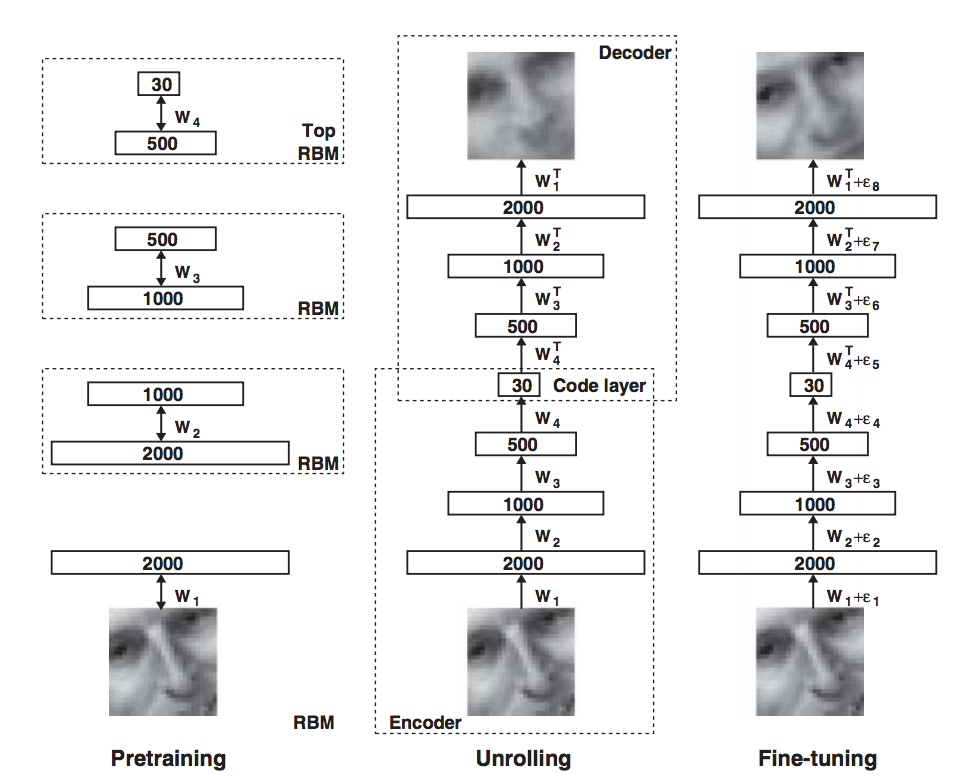
\includegraphics[scale=0.5]{images/DBN-RBM-process.png}
 \caption{The Autoencoder training steps \cite{Hinton2}}
 \label{figure-DBN-RBM}
 \end{figure}
 
\subsubsection {Stacked Denoising Autoencoders}\label{SDAE}

 The second important piece of work was the development of a denoising autoencoder (DAE), by Vincent  et al. \cite{Vincent}. 
 One of the problems identified in the DBN model (and those similar), is that if the encoder dimensions were too high, 
 it is likely that the encoder would learn a trivial encoding - essentially creating a “copy the input” model. The one way
  of tackling this issue is to constrain the representation with bottlenecks and sparse autoencoder layers, which can be seen in figure  \ref{figure-DBN-RBM}.
  \hfill \break 

Vincent et al. explore a very different approach to the problem, which was to develop an implementation of 
autoencoder which focused on partially corrupting the input, and so force the network to ‘denoise’ it. The theory 
here is based on two ideas - the first, is that a higher dimensional representation should be robust to partial 
corruption of the input data; and the second is that the denoising process will force model focus to shift to 
extracting useful features from the input.
 \hfill \break 

The algorithms and structures are largely the same as described for DBNs above, with the key difference 
being that the model is trained to reconstruct the original input, but only using a corrupted version of the input 
(where noise has been added to it), and so is forced to learn smarter feature mappings and extractions. 
The DAE suggested then is a stochastic variant of the autoencoder, which has the benefit of being able to 
implement higher dimensional representations without risking training of a trivial identity mapping. Notably, 
in the Stacked Denoising Autoencoder (SDAE) formation, only the initial input is corrupted (as opposed to the 
input from layer to layer). It was shown that the SDAE model outperformed previous AE and DBN networks on 
numerous benchmark datasets \cite{Vincent} . 

\subsubsection {Pre-training}

The methods described above follow a similar approach: greedy layer-wise unsupervised pre-training in order to 
determine initial weights, followed by supervised fine tuning to arrive at the final model. It is shown numerous times, 
that the pretraining process results in significant performance gains \cite{Vincent}. However it is not immediately apparent, 
given the nature of backpropagation algorithms and the like, why this is the case. Erhan et al. performed 
extensive empirical simulations in order to suggest an explanation to the mechanism of pre-training \cite{Erhan}.
 \hfill \break 

While their results were not entirely conclusive, they did lend themselves to a reasonable hypothesis: 
the unsupervised pre-training results in a form of regularization on the model - variance is minimized, and the 
bias introduced acts as a prior to direct the model configuration towards a sample space that is effective for the unsupervised 
learning generalization optimisations.

\subsubsection {Time Series Applications}

The autoencoder papers reviewed so far in this section derive their results primarily from classification problems, 
and so do not necessarily account for the problems involved with time series as described in \ref{HDDR}. Due to 
the inherent difficulties with predictions in the financial system, it can sometimes be unclear if the shortcoming in 
results is due to this system complexity or if the methodologies used are unsuited for the purpose. In light of this 
it is worth pointing out that Stacked Autoencoder (SAE) implementations have been shown to be effective in many
 time series systems.  
 \hfill \break 

Lv et al.  implemented a deep learning SAE model using the methods described in \ref{SDAE} in order to 
predict traffic flow at various time intervals (15, 30, 45 and 60 minutes) - a problem not so structurally dissimilar 
from what will be presented in this paper \cite{Lv}. They were able to show that the deep SAE was able to offer prediction 
results which were both objectively good and also persistently outperformed the comparison models used 
(backpropagation neural network, random walk forecast, support vector machine and a radial basis function 
neural network).
\hfill \break 

In a review of unsupervised feature learning and deep learning methods on time series, Langkvist et al. noted that 
the use of autoencoders, either as a technique in themselves, or as an auxiliary technique to models 
such as convolutional neural networks, were able to offer performance increases in areas such as video analysis, 
motion capture data and bacteria identification \cite{Langkvist}.
 
\subsubsection{Financial Applications}

There have of course also been successful applications of stacked autoencoders and deep learning models in 
finance as well. Takeuchi et al. performed some earlier work showing the use of autoencoders when applied to a 
momentum trading strategy. They implemented an RBM pre-trained DBN as per \ref{DBN}, and assessed the 
networks classification performance for ordinary shares on NYSE, AMEX and Nasdaq. This showed that using a 
DBN network resulted in significant performance increases compared to the standard momentum strategy \cite{Takeuchi}.
\hfill \break 

Zhao et al. used SDAEs and combined them with the bootstrap aggregation ensemble method (‘bagging’) in a 
study of predicting the crude oil price. They compared the proposed model to a variety of benchmarks, including 
standard SAE, bagged and standard feedforward networks and SVRs. The results indicated that the SAE models 
were more accurate, with the bagged SAE model performing the best, though at a significant increase in 
computational costs in comparison to standard SAE \cite{Zhao}.
\hfill \break 

While much of the financial literature has focused on the use of RBM based models, Autoencoders and SAEs have 
recently been gaining popularity in performing feature reduction. Troiano et al. specifically investigate the use of 
different feature reduction models for trend prediction in finance \cite{Troiano}. In line with being primarily 
interested in the effect of feature reduction techniques, rather than the classification performance itself, only an 
SVM model was used to test results. Using various periods from historical S\&P 500 data, they were able to show 
that AE outperformed the RBM model significantly in numerous accuracy measures, and was able to do so at a 
fraction of the training time.
\hfill \break 

Bao et al.  note that the research has been lacking with regards to whether SAEs should be used for 
financial prediction models or not \cite{Bao}. They suggest a novel model which combines Wavelet Transformation, SAEs 
and a Long Short Term Memory (LSTM) network. Using data from several financial exchanges (considering a 
range of ‘developed’ and ‘undeveloped’ markets), they assess the model’s applicability to OHLC prediction. 
Comparing the model to configurations without the SAE layers, and a RNN model as benchmark, they showed 
that the inclusion of SAEs resulted in less volatility and greater accuracy, which in turn offered higher profitabilities 
in a buy-and-hold trading strategy.
\hfill \break 

More novel autoencoder applications have also been attempted, with Hsu suggesting the use of a 
Recurrent Autoencoder for multidimensional time series prediction \cite{Hsu}. There is a clear pattern through the literature 
that the use of AEs and SAEs both by themselves and when used as an assisting technique result in more accurate 
prediction results and less computationally expensive training.

\subsection{Data Segmentation}
\hfill

One of the aspects of time series not yet discussed is how the data might be segmented for analysis. 
Financial pattern matching, as discussed in \ref{TechnicalAnalysis}, requires methodologies to decide the length of data to 
consider when determining whether a subset of data matches a pattern or not. 
\hfill\break

There are numerous classical approaches to this problem, which were widely applied in machine learning prior to 
the resurgence in deep learning. One of the earliest and more common approaches was the ‘Sliding Window’, 
where each the model input for each observation is ‘padded’ by a predetermined number of observations that 
occurred both prior and after the one in question. This has the advantage of being fairly model agnostic, but fails 
to capture any correlations in the dependent variable values \cite{Chu}. The Recurrent Sliding Window method 
aims to resolve this by including the same number of prior predictions made as part of the input. In this case, input 
would be ${<x_{t-d},...x_{t},…,x_{t+d}> and <y_{t-d},...,y_t>}$. This was shown to be significantly more effective than the plain 
sliding window method \cite{Bakiri}. Notably, the sliding window approach can only be implemented in an offline 
model.
\hfill\break

These methods can be adapted to take on online formats, as well as incorporate data reduction benefits 
through algorithms such as Piecewise Linear Approximation (PLA), which adapts a linear representation to the 
leading portion of the window. Some novel approaches (Feasible Space Window and it’s stepwise adaption) were 
suggested by Liu et al. in order to compensate for the computational requirements of reprocessing the entire 
window at each step for online models \cite{Liu}.
\hfill \break 

Window based methods represent a fairly static and unsophisticated approach to data segmentation. 
A suggested solution to this is to segment the data by dynamically identifying significant partition points, 
known as perceptual important points (PIP) \cite{Chung}. The computational cost of identifying PIPs was initially 
rather large, making them unsuitable for quickly changing and dynamic environments such as finance. 
However, Zhou et al. suggested a novel approach which reduced computational costs through intelligent binary 
tree traversal. They were able to show this approach was effective in identifying traditional financial stock patterns 
with the use of a layered neural network \cite{Zhou}. In a similar fashion, input data turning points (TP) were shown to 
potentially offer lower error rates than PIPs by Yin et al. \cite{Yin}.
\hfill \break 

More recently, Wan et al. conducted a review on the effect of segmentation on financial time series pattern 
matching, comparing perceptual important points, piecewise aggregate approximations, piecewise linear 
approximations and turning point based methods \cite{Wan}. They use several pattern matching algorithms 
(template-based, rule-based, hybrid, decision tree, and symbolic aggregate approximation) for each of the 
segmentation methods in order to determine their effect on a broader level. The analysis was performed on real 
stock market data, as well as synthetic data generated to display common patterns such as positive/negative 
head and shoulders (H\&S). Measuring accuracy, precision and recall, they showed that PIP based segmentation 
generally offered superior results to the others (though it is worth noting that there were various performance 
differences within the segmentation methods depending on the matching algorithm used).

\subsection{Online Learning Algorithms and Gradient Descent} \label{lr_OGD}
\hfill

Most classic machine learning algorithms operate under the assumption that, for all intents and purposes, the 
full dataset has been collected and that the amount of training data for the model is both finite and immediately 
available. However, as the growth of information grows in an exponential fashion, there are numerous areas where
 the expected training data for the model will continue to grow. In these cases it would be disadvantageous to go 
 through the full training and validation process again in order to incorporate the newly available data.
\hfill\break

Online algorithms are designed to offset these issues by adjusting the batch training technique to rather 
repetitively draw on single samples from the data on which the model’s parameters can be adjusted. The benefit 
is that they are able to quickly process a large number of observations and readjust the model, though the 
downfall is that they are not always able to optimize the cost function to the same extent as offline batch 
algorithms \cite{Albers}.
\hfill\break

Bottou and Cun argue that as the size of the dataset grows significantly, online algorithms advantages result in 
them outperforming offline models, despite any initial drawbacks \cite{Bottou}. Previous research had shown that online 
algorithms typically perform as fast as batch algorithms during the ‘search’ phase of parameter optimization, but 
that ‘final’ phase convergence tended to fluctuate around the optima due to the noise present in single sample 
gradients \cite{LeCun, Bottou2}. Bottou and Cun showed in fact, that it is more practical to consider the convergence towards
 the parameters of the optima, rather than the optima itself (as defined by the cost function) - the difference 
 between the learning speed and optimization speed, respectively \cite{Bottou}. Theoretical and empirical findings were 
 presented to show that a stochastic online gradient descent (SGD) algorithm \textbf{[referenceappendix] }was able to 
 outperform the batch model for parameter estimation, and was able to asymptotically outperform in the number of 
 samples processed in a time period. The stochastic aspect of the algorithm is related to random observations 
 from batch sample groups being used as the gradient basis. Theoretically, this slows down the convergence, but 
 speeds up the processing speed of each batch - a technique which has later been shown to be generally 
 successful \cite{Shalev, Zhang}. 
 \hfill\break
 
 The SGD algorithm has resulted in a fair amount of further research due to its applicability to machine learning 
 and the online benefit, which can largely be group into two categories: improvements affecting gradient learning 
 and convergence rates, and processing improvements through parallelization.
\hfill\break
 
 One of the earlier improvements to convergence rates was the Momentum algorithm, as developed by Tseng \cite{Tseng}. 
 As noted, stochastic descent often introduces significant oscillation around an optima, which slows down 
 convergence. Momentum reduces this by decreasing movement in directions of high curvature, and increasing 
 increasing movement towards directions consistent with previous gradients (this is achieved through combining 
 gradient movements in opposite directions) .
\hfill\break

There have also been several attempts to introduce effective regularization into the SGD process. Bartlett et al. 
presented Adaptive Online Gradient Descent, which implements an adaptive step size through a $\lambda$ 
penalty on the learning rate, which was shown to be nearly optimal in a strong sense \cite{Bartlett}. Langford et al. 
demonstrated a variation named Truncated Gradient, which introduced an enforced weight sparsity parameter. 
The weight sparsity is able to achieve equitable effects to $L_1$ regularization (similar to Lasso Regression). 
They were able to show that implementation performed effective feature reduction, while having little effect on 
performance \cite{Langford}. Other approaches, such as AdaGrad, aim to improve the robustness of gradient training by 
adjusting the updates to parameters according to frequency - e.g. larger updates to infrequent parameters, and 
smaller updates to frequent parameters \cite{Duchi, Zeiler}. 
\hfill\break

A parallel implementation of SGD largely rests on the idea of splitting up data to be processed in individual runs 
of the gradient descent. The results are periodically aggregated, and the new model parameters are distributed 
to processing nodes for further training \cite{Zinkevich}. Depending on the configuration, the variance within results can 
result in poor convergence rates \cite{Mahajan}. Mahajan et al. suggest a novel implementation which improves the 
distribution impacts through the use of better approximating functions in the processing nodes, which in turn 
improves the efficacy of the algorithms convergence \cite{Mahajan}. Povey et al. presented a Natural Gradient SGD, 
which improves the learning rates through the use of a factor matrix used on the new gradients. They were able 
to show empirical evidence of this improving performance issues introduced from the parameter averaging 
typically used in parallelization \cite{Povey}.
\hfill\break

There have been some more recent improvements focusing on making the SGD algorithm more dynamic, 
including the Inconsistent SGD (ISGD) and AdaBatch adaptations. The idea behind ISGD is to treat the training 
on a particular batch as a stochastic process, and adjust it according to the expected loss identified. Gradient 
updates from small loss batches are relatively small compared to large loss batches, and so by focusing efforts 
here ISGD is able to optimize performance. Wang et al. performed careful testing of SGD vs. ISGD and found 
inconsistent training to consistently outperform in terms of convergence speed and results \cite{Wang}. It is worth 
noting that due to its nature, ISGD can be effectively combined with other SGD improvements (e.g. Momentum, 
as per the authors’ experiments). AdaBatch, as presented by Devarakonda et al., introduces dynamism through 
the adjustment of batch sizes. Small batch sizes in SGD offer the benefit of faster convergence in fewer training 
epochs, however larger batch sizes are more computationally efficient due to their applicability to parallelization. 
The algorithm uses a monotonically increasing batch size, which is started small to gain traction in convergence, 
and later increased to allow the benefits of data parallelism. The effect, as shown, is to offer improvements in 
training performance of up to 6x, with less than 1\% of accuracy when compared to the fixed batch baselines \cite{Devarakonda}. 
Both of these algorithms have been shown to be effective and applicable in the context of online neural network training.
\hfill\break

\subsection{Backtesting and Model Validation} \label{lr_backtesting}
\hfill

Much of financial academic literature is currently facing a problem in terms of validation and verification of results. 
The primary method of going about these ends in the past has been to perform historical simulations, or ‘backtests’ ,
in order to prove profitability of a trading strategy. The recent advances in both technology and the algorithms available 
to construct these strategies has resulted in researchers being able to run so many iterations of a model or strategy
 configuration through these backtests, that its become increasingly difficult to control for spurious results, with some 
 papers suggesting that ‘most published research findings are false’   \cite{Ioannidis}.
\hfill \break 

The standard way of implementing backtests is to split the data into two portions: an In Sample (IS) portion which
 is used to train the model, and an Out of Sample (OOS) portion which is used to test the model and validate results. 
 The problem lies in that millions of different model configurations might be tested, and if more sophisticated test 
 measures are not in place (i.e. not just the standard Neyman-Pearson hypothesis testing framework is implemented), 
 then it is only a matter of time before a false positive result occurs which shows high performance both IS and OOS (i.e. overfitting). 
 The nature of financial data, where there is a low signal-to-noise ratio in a dynamic and adaptive system, and 
 where there is only one true data sequence, makes it difficult to resolve these issues effectively 
\cite{BailyPBO, McLean}.
\hfill \break 

Overfitting is not a novel issue, and has of course been tackled in various literature areas, including machine learning. 
However, in that context, the frameworks are often not suited to the buy/sell with random frequency structure of 
investment strategies. They also do not account for overfitting outside of the output parameters, or take into 
consideration the number of trials attempted. Other methods, such as ‘hold-out’, are arguably still faulty due to researcher 
knowledge while constructing models \cite{Schorfheide}. One of the downfalls of the typical IS-OOS set up in the 
financial context is also that the most recent (and relevant) data will not be able to be used for the model training. 
\hfill \break 

There have been some suggestions to resolve the problem that is occuring in the literature as a result of this - some 
work suggesting new frameworks, which this section will cover, and others which focus on the review process or 
how data and replication procedures are made available \cite{Prado}. While the points made with regard to the review process 
and so on are certainly important, they don't aid with more effective model training for the researcher up front, and 
so will not be covered here.

\subsubsection{Testing Methodologies}\label{lr_cscv}

Considering the issues laid out above, there has been much work to develop alternative approaches to backtesting. 
One of the common approaches to avoid backtest overfitting is the ‘hold-out’ strategy, where a certain portion of 
the dataset is reserved for testing true OOS performance. Numerous problems have been pointed out with this 
approach, including that the data is often used regardless, or that awareness of the movements in the data may, 
consciously or otherwise, influence strategy and test design by the researchers \cite{Schorfheide}. For small samples, 
a hold-out strategy may be too short to be conclusive \cite{Weiss}, and even for large samples it results in the 
most recent data (which is arguably the most pertinent) not being used for model selection \cite{Hawkins, BailyPBO}.
\hfill \break 

There has been work by several authors to try and lay out techniques to try and avert backtest overfitting. 
The Model Confidence Set (MCS), as developed by Hansen et al. \cite{Hansen}, starts with a 
collection of models or configurations, and remove models iteratively according to a defined loss function. 
The confidence set is defined by the remaining models once a non-rejection takes place within the process, and 
these models are considered to be statistically similar within a certain confidence range. MCS is thus able to facilitate 
equitable model selection. However, Aparicio et al. \cite{Aparicio}, showed  that while MCS is a potential strategy, in 
practice is is ineffective due to the inordinate requirement of signal-to-noise necessary to identify true superior 
models, as well as a lack of penalization over the number of trials attempted.
\hfill \break

Bailey et al. \cite{BailyPBO} have developed a more robust approach to backtesting and how overfitting during strategy 
selection might be avoided, called Combinatorially Symmetric Cross-validation (CSCV). Their research defines backtest overfitting as having occurred when the strategy selection which maximizes IS performance systematically underperforms median OOS in comparison to the remaining configurations. They use this definition to develop a framework which measures the probability of such an event occuring, where the sample space is the combined pairs of IS and OOS performance of the available configurations. The probability of backtest overfitting (PBO) is then established as the likelihood of a configuration underperforming the median IS while outperforming IS. 
\hfill \break 

The CSCV methodology provides several important benefits over traditional testing 
frameworks, including the usual K-fold cross validation used in machine learning. By recombining the slices of 
available data, both the training and testing sets are of equal size, which is particularly advantageous when comparing 
financial statistics such as the Sharpe Ratio (SR), which are susceptible to sample size. Additionally, the symmetry 
of the set combinations in CSCV ensure that performance degradation is only as a result of overfitting, and not 
arbitrary differences in data sets. It is pointed out that while CSCV and PBO should be used to evaluate the quality 
of a strategy, they should not be the function on which strategy selection relies, which in itself would result in overfitting.
\hfill \break 

\subsubsection{Test Data Length}

The CSCV methodology offers an important but highly generalised framework to assess models and backtest 
overfitting. It doesn’t however indicate which metrics should be used to assess the IS and OOS performance, nor 
any indication on the amount of data needed to do so effectively. One of the noted limitations of the framework is 
that a high PBO indicates overfitting within the group of N strategies, which is not necessarily indicative that none 
of the strategies are skillful - it could be that all of them are. Also, as pointed out, it should not be used as an 
objective function to avoid overfitting, but rather as an evaluation tool. To this end it helps assess overfitting, but 
not necessarily avoid it. 
\hfill \break 

A typical measure of evaluation used for financial models is the Sharpe Ratio (SR), which is the ratio of between 
average excess returns and the returns’ standard deviation - a measure of the return on risk. In the context of 
comparing models, SR is typically expressed annually to allow models with different frequencies to be compared. 
Lo et al. \cite{Lo} show that annulaized SR can be expressed as

\begin{equation}\label{SRAnnual}
SR=\frac{\mu}{\sigma}\sqrt{q}
\end{equation}

Using sample means and deviations, $\hat{\mu}$ and $\hat{\sigma}$, SR can be shown to converge as follows 
(as y $\rightarrow\infty$)

\begin{equation}\label{SRConvergence}
  \hat{SR}  \rightarrow \mathcal {N} [SR,\frac{1 + \frac{SR^2}{2q}}{y}]
\end{equation}

Thus, when using SR estimations, which follow a Normal distribution, it is possible that where the true SR mean is 
zero we may still (with enough configurations attempted) find an SR measurement which optimises IS performance. 
This is shown by Bailey et al. \cite{BaileyBTL}, who propose the non-null probability of selecting an IS strategy with null expected 
performance OOS. Notably, typical methods such as hold-out once again fail, as the number of configurations 
attempted are not recorded. They add a further derivation, thich is the Minimum Backtest Length (MinBTL), ultimately 
showing that

\begin{equation}\label{MinBTL}
MinBTL \approx (\frac{
                                  (1-\gamma)Z^{-1}[1-\frac{1}{N}] + \gamma Z^{-1}[1 -\frac{1}{N}e^{-1}]}
                                  {\overline{E[max_N]}})^2
                                  < \frac{2ln[N]}{\overline{E[max_N]}}^2
\end{equation}

The statistic highlights the relationships between: selecting a strategy with a higher IS SR than expected OOS, 
the number of strategies tested (N), and the number of years tested (y). The equation shows that  as the number 
of strategies tested increases, the minimum back test length much also increase in order to contain the likelihood 
of overfitting to IS SR. 
\hfill \break 

As shown extensively throughout ML literature, increased model complexity and number of parameters is one of 
the primary causes of overfitting. In context of the MinBTL formula, model complexity affects the number of 
configurations that are available and which may be tested, which in turn will increase likelihood of overfitting. 
A lack of consideration, or reporting, of the number of trials makes the potential for overfitting impossible to assess. 
\hfill \break 

Bailey et al. expanded on this view with assessing the impact of presenting overfit models as correct. 
They were able to show that in lieu of any compensation effects (i.e. a series following a Gaussian random walk), 
there is no reason for overfitting to result in negative performance. However, where compensation effects apply 
(e.g. economic/investment cycles, bubble bursts, major corrections etc.), then the inclusion of memory in a strategy
 is likely to be detrimental to OOS performance if overfitting isn’t controlled for \cite{BaileyBTL}.
\hfill \break 

\subsubsection {Sharpe Ratio}

The use of the Sharpe Ratio in financial backtesting is not just an arbitrary or persistent literature choice. 
The statistic offers two benefits: the effectively strategy-agnostic financial information contained, as well as being 
relatable to the t-statistic, and so simple to perform hypothesis testing. The SR ratio (estimate from sample as $\hat{SR}$) 
is defined as

\begin{equation}\label{SR}
  SR=\frac{\mu}{\sigma}
\end{equation}

The t-ratio is defined as 

\begin{equation}\label{tratio}
  t-ratio = \frac{\hat{\mu}}{\hat{\sigma}/\sqrt{T}}
\end{equation}

Evidently, the link heree ratio (though it can be generalized to another statistic with a probabilistic interpretation). Additionally, 
PBO is generally more in line with machine learning literature with the cross validation like approach on time series data.  
\hfill \break 

It should be noted, that the literature detailing usage of the Sharpe ratio for strategy comparison is extensive, with 
numerous variations and methodologies offered \cite{BaileySharpe}. However, the crux of this paper lies 
in whether an online neural network is able to make effective enough predictions that a strategy might use the 
predictions to be profitable. The subtlety here is that we will consider the usage of such forecasting \textit{within} a strategy,
 rather than \textit{as} a strategy itself. In line with this, statistics such as the Sharpe ratio will be used, but not form a critical 
 consideration of the research here as the comparison of strategies used will be a secondary concern.
\hfill \break 

\newpage


\section{Data}\label{Data}
\subsection{Data Processing}

The datasets used go through several transformations throughout the usage cycle, each of which are captured below.

\subsubsection{Log Difference Transformation and Aggregation}\label{ldata_og_difference}
All datasets were transformed into log feature fluctuation values, and were then expanded to include fluctuations over rolling window periods.
\begin{equation}
\textit{log\_diff}(x_t) = ln(x_t) - ln(x_{t-1})
\end{equation}
This log feature fluctuation,  is processed for each OHLCV feature and for each time point (from the previous time point). The log fluctuations have the benefit of taking compound effects into account in a systematic way and symmetric in terms of gains and losses.
\newline\newline
The datasets are then expanded with the rolling window summations both in the past, for input, and in the future, for predicted output. For example, at each data point $t$, the following time series are added:
\begin{itemize}
	\item [$\cdot$] Log feature fluctuations over the periods $(t-5, t)$ and $(t-20, t)$ (with $(t-1, t)$ already having been processed)
	\item [$\cdot$] Log feature fluctuations for the period $(t, t + 2)$, to be predicted \todo{Change to final windows decided on}
\end{itemize}

Only data points with a full set of features are used for training and prediction later on in the framework.

\subsubsection{Data Scaling}\label{data_scaling}
Once the log difference data has been processed, the datasets are either standardized or normalized to allow for better learning. This is done in the typical ways:
\begin{equation}
\textit{standardize:  }x_s = \frac{(x_i - \bar{x}) }{\sigma_x}
\end{equation}

\begin{equation}
\textit{normalize:  }x_n = \frac{x_i - min(x) }{max(x) - min(x)}
\end{equation}

Two extensions of these are used later on, dubbed 'Limited Standardization' and 'Limited Normalization', which are used when the data is split up into the SAE training and OGD prediction sets. In this case all the data needs to be scaled, but the information should not be travelling from the OGD dataset to the SAE training set through the use of aggregated measures such as $\bar{x}$. Thus, if the data is split at point $t$ out of $n$ data points, the scaling would be implemented as follows:

\begin{equation}
\textit{limited standardize:  } x_{ls} = \frac{(x_i - \bar{x_{1:t}}) }{\sigma_{x_{1:t}}} , \forall  i \in (1, n)
\end{equation}

\begin{equation}
\textit{limited normalize:  } x_{ln} = \frac{x_i - min(x_{1:t}) }{max(x_{1:t}) - min(x_{1:t})} , \forall  i \in (1, n)
\end{equation}


This log-differenced, aggregated and scaled data is then used as the input for the neural network models.

\subsubsection{Reverse Data Scaling}\label{data_reverse_scaling}

The predicted data points are transformed back into actual prices for returns analysis. The first step is to reverse the scaling that is done in \ref{data_scaling} in order to retrieve the log difference fluctuations.

\begin{equation}
\textit{reverse standardize:  }x_i = x_s * \sigma_x + \bar{x}
\end{equation}

\begin{equation}
\textit{reverse normalize:  } x_i = x_n * (max(x) - min(x)) + min(x)
\end{equation}

These are applied similarly for the limited variations.

\subsubsection{Price Reconstruction}\label{data_price_recon}

The predicted log fluctuations produced in \ref{data_reverse_scaling} are used to reconstruct the predicted prices. For original prices $o$, stocks $s$, time window predicted $t$, predicted log fluctuation $p$ and time steps $i \in (0, n)$i:

\begin{equation}
\textit{reconstructed price}_{s,i} = o_{s,i-t} * e^{p_{s,i}}
\end{equation}

These reconstructed prices are then used to assess model returns later.

\subsection{Synthetic Data}\label{data_synthetic}

Synthetic datasets were generated to represent known trends with some variance in prices. Geometric Brownian motion was used to simulate stock price movements. Each dataset was generated with a random seed (using a Mersenne Twister pseudorandom number generator), and had a structure of 9 stocks:

\begin{itemize}
	\item [$\cdot$] 2 stocks with an upward trend, and high and low variance levels
	\item [$\cdot$] 2 stocks with a downward trend, and high and low variance levels
	\item [$\cdot$] 2 stocks with a sideways trend, and high and low variance levels
\end{itemize}

The steps for Geometric Brownian Motion are described in \ref{algo_brownianmotion}, which allows the stocks simulations to be implemented with a trend ($\sigma$) and variance ($\mu$) for each stock.\newline

\RestyleAlgo{algoruled}
\begin{algorithm}[H]
	\KwIn{$\sigma$, $\mu$, $S_0$, $steps$}

	t = 1/steps\;
	prices = [$S_0$]\;

	\ForEach{i in 1:t}
	{
		z = random()  $\sim N(0,1)$\;
		$S_t = S_{t-1}*e^{(\mu - \frac {\sigma^2}{2})t + \sigma  \sqrt{t}  z)}$\;
		prices = [prices; $S_t$]\;
	}
	\KwResult{prices}
	\label{algo_brownianmotion}
	\caption{Geometric Brownian Motion Simulation}
\end{algorithm}

\paragraph{Simulated Dataset}

This section will detail the chosen $\sigma$ and $\mu$ values for the dataset, as well as the expected results from training on them.\todo{finish this}


\subsection{Real Data}

This section will detail the use of real data - namely the JSE ALSI data collected, and the time periods collected for. Detail will be added once this dataset has been finalised. \todo{finish this}

\newpage
\section{Implementation}\label{Implementation}
\subsection{Process Overview}\label{ProcessOverview}\label{imp_overview}


The implementation focuses on bringing together several ideas: data reduction, deep learning with pre-training/weight initialization, online learning and backtest overfitting validation for the purposes of stock price prediction. The process implementation is discussed fully in \ref{imp_fullprocess}, but can be summarised as the following:

\begin{itemize}
	\item [1] The dataset is split into 2 subsets: the SAE/FFN  portion, and the OGD portion
	\item [2] The first subset is used to train the SAE and deep FFN using the SGD algorithm. These networks were implemented with pre-training and weight initialization techniques
	\item [3] The second subset of data is used to continue training the network in an online manner using OGD
	\item [4] The returns generated from OGD can then be used in the CSCV process, to estimate the probability of backtest overfitting
\end{itemize}
~\\
The rest of this chapter will detail the algorithms used to train the relevant FFN, RBM and SAE networks, as well as the trading strategy and CSCV \& PBO testing procedures.

\subsection{Feedforward Neural Networks}\label{imp_ffn}
~\\
Feedforward Neural Networks (FFN) in the form of multilayer perceptrons is a well established network technique, providing effective nonlinear representations for both shallow and deep structures \cite{Schmidhuber}. Specifically, a FFN is made up of several non-cyclical layers: the first and last are the input and output layers, respectively, and any inbetween are referred to as 'hidden' layers. Each layer is made up of nodes which are fully connected to the nodes in the previous and following layers, but does not have connections to nodes within the layer - information only travels forward. Each 
node has an activation function, which acts on the weighted input from the previous layers' nodes.

\subsubsection{Notation and Network Representation}\label{imp_ffn_functions}

\begin{itemize}
\item[$\cdot$] The weights from the $j^{th}$ node in the $l^{th}$ layer from the $k^{th}$ node in the $(l-1)^{th}$ layer are represented by $w^l_{jk}$
\item[$\cdot$] The bias for the $j^{th}$ node in layer $l$ is represented by $w^l_0j$
\item[$\cdot$] The output for the $j^{th}$ node is defined as $o(z_j)$, for an activation function $o$ and weighted input $z$
\item[$\cdot$] The weighted input for the $j^{th}$ neuron in a layer is $z^l_j=\sum_{n=i}{a^{l-1}_iw_{ij}} + w_{0j}$
\end{itemize}
~\\
These definitions allow an input into the network to be propagated through it, having the original values processed through the weights and activations functions, and have an output in the form of the network's last layer.

\subsubsection{Activation Functions}
~\\
As noted in \ref{lr_activationfunctions}, there are 3 primary characteristics of concern for activation functions: non-linearity, continuous differentiability and monotonicity. While many different functions have been suggested and used, 2 of the most used were implemented here.

\subparagraph{Sigmoid}

The sigmoid, or logistic, function is one of the most popular and widely used activation functions historically, and is defined as 
\begin{equation}\label{func_sigmoid}
f(x) = \frac{1}{1 + e^{-x}}
\end{equation}

The Sigmoid function is in the range [0,1], making it a suitable choice for problems requiring a probabilistic output. The slope of the function curve is both a boon and a drawback: it allows for fast learning initially, but results in learning slowdown later (often casuing what is referred to as node 'saturation'). The exponent calculation is also computationally expensive, relatively speaking.

\subparagraph{ReLU}

The Rectified Linuear Unit (ReLU) is, as discussed in \change{needs reference section}, a newer activation function which has been shown to be effective in deep learning networks. It is defined as

\begin{equation}\label{func_relu}
f(x) = max(0, x)
\end{equation}

The function has the benefits of quick learning which doesn't saturate, as well as being computationally cheap. The downside is that the non-gradient for the negative range of the function can result in 'dead' nodes, which stop updating with the learning process (though 'Leaky ReLUs' can be used to help resolve this)

\subsubsection{Backpropagation}\label{imp_backprop}

The backpropagation algorithm, as discussed in \ref{lr_trainingbackprop}, has allowed for effective training of FNNs for given data. The algorithm relies on incremental improvements of the model, as defined by decreasing the cost function. A common choice for cost is Mean Squared Errors (MSE):

\begin{equation}\label{function_MSE}
C = \frac{1}{2} \rVert y - a^L \rVert^2
\end{equation}
~\\
This allows the backpropagation algorithm to implemented as follows:

\begin{itemize}
	\item[$\bullet$]  Let N be a neural network of weights \textit{w}, inputs \textit{x} and outputs \textit{y}, where the weights are (naively) initialized to random values
	\item[$\bullet$] The algorithm then iterates through the following:
	\begin{itemize}
		\item[1] Select a set of $m$ samples $x_s$
		\item[2]Forward Pass:
		\begin{itemize}
			\item[i] Propagate the samples through the network using the functions defined in \ref{imp_ffn_functions} to generate out output $y_s$
			\item[ii] Calculate the error term (aka cost), as
			\begin{equation}
				\lambda^L_x = \nabla_a C \otimes o'(z^L) = (a^L - y) \otimes o'(z^L)
			\end{equation}
		\end{itemize}
		\item[3]Backward Pass:
		\begin{itemize}
			\item[i] Propagate activation value back through the network to calculate the delta values (the difference between the network outputs and desired output values at each layer)
			\begin{equation}
			\lambda^l_x = ((w^{l+1})^T\lambda^{l+1})  \otimes o'(z^l)
			\end{equation}
			\item[ii] Each weights output delta and input activation are multiplied to find the weight’s gradient and this gradient is reduced by a factor of the ‘learning rate’ $\eta$, and the mean of this is subtracted from the network weights
			\begin{equation}
			w^l \rightarrow w^l - \frac{\eta}{m} \sum_{x} \lambda^{x, l} (a^{x, l - 1})^T
			\end{equation}
		\end{itemize}
		\item[4] Repeat from step 1, unless a minima or other stopping criterion is reached
		
	\end{itemize}
\end{itemize}

\subsubsection{Gradient Descent Algorithms}\label{imp_sgd}

Stochastic Gradient Descent (SGD), as discussed in \ref{OGD}, has been shown to increase the speed at which the backpropagation algorithm can converge a minima in terms of cost. The algorithm runs backpropagation over the entire dataset for a number of 'epochs', and updates the network incrementally through the epoch. The stopping condition for the algorithm is usually defined as either a particular number of epochs being reached, or cost no longer decreasing for some number of epochs (i.e. a minima has been reached).

\begin{itemize}
	\item [$\cdot$] For each epoch:
	\item [1] Select $k$ samples at random from the data which have not yet been sampled in this epoch
	\item [2] Use backpropgation on the network using the $k$ samples to update the weights
	\item [3] Repeat 1-2 until all samples from the dataset have been sampled
	\item [4] Start a new epoch, or finish if a stopping condition has been reached
\end{itemize}

Where SGD is appropriate and effective for scenarios where the entire dataset is available, Online Gradient Descent (OGD) is applicable for when the model is learning in an online fashion. In this case, the backpropagation is run as defined above, but for only one sample at a time (i.e. $m=1$)

\subsubsection{Gradient Descent Improvements}\label{imp_gradientimprovements}

This section will detail and improvements that are used in the project - i.e. L1 and L2 regularization, or the learning rate schedule \todo{write this section}

\subsection{Restricted Boltzmann Machines}\label{imp_rbm}

Restricted Boltzmann Machines (RBM) are generative networks which can be trained to learn probability distributions over a dataset. They are structurally different from a FFN in that they have a recurrent weight function - a typical RBM has one visible layer (input/output), and one hidden layer. A sample will be processed from the input layer to the hidden layer, and the activation values from the hidden layer will be used by the input layer to provide a recontruction. The hidden units thus correspond to feature detection of the visible unit data structures, and the learning process of the network results in effetive parameter estimation. 

One of the primary differences from an FFN lies in the stochastic unit determination - the values in a hidden layer will typically be implemented such that the take on a binary value with a probablistic likelihood. Thus, the input and output have the same structure, and the processing from the hidden layer creates the generative process learned by the RBM. 
~\\
The joint configuration $(v,h)$ of the visible and hidden units has an energy \todo{add Hopfield 1982 ref} given by:

\begin{equation}\label{func_rbmenergy}
E(v,h) = - \sum_{i \in visible} a_iv_i - \sum_{j \in hidden} b_jh_j - \sum_{i,j}v_ih_jw_ij
\end{equation}

where $v,h$ correspond to the binary states of the visible and hidden units, with biases $a,b$, and weights $w$. It can be shown \todo{add hinton reference TR guide}, that network weights can be adjusted to change the probabilities assigned to a particular training sample. The derivations of \ref{func_rbmenergy} show that performing a stochastic asent for the log probability of the data can be implemented through the following weight adjustment:

\begin{equation}
\Delta w_{ij} = \eta (\langle v_ih_j\rangle_{data} - \langle v_ih_j\rangle_{model})
\end{equation}

The angular brackets here indicate expectations under the distribution specified by the following subscript. Due to the probabilistic nature of RBMs, the [0,1] ranged Sigmoid activation function is typically used. Thus, for hidden nodes and a data sample $v$, the it is easy to get unbiased sampling of $\langle v_ih_j \rangle_{data}$

\begin{equation}
p(h_j=1) = \sigma(w_{0j} +  \sum_{i=1}v_iw_{ij})
\end{equation}

Similarly, the visible states (or reconstruction), can then be calculated as 

\begin{equation}
p(v_i=1) = \sigma(w_{0i} + \sum_{j=1}h_jw_{ij})
\end{equation}


Getting an unbiased sample of $\langle v_i h_j \rangle$ proves more problematic, and so the model reconstructioms via Gibbs sampling are used instead (this is explained below), resulting in the weight updates of

\begin{equation}
\Delta w_{ij} = \eta (\langle v_ih_j\rangle_{data} - \langle v_ih_j\rangle_{reconstruction})
\end{equation}

While it's important for the hidden units to take on a binary value (and so avoid communicating real values rather than learning structure), the visible units may be chosen to take on the probability values, rather than the stochastic samples, particularly if real valued output is necessary. 

\subsubsection{Contrastive Divergence}\label{imp_CD}

The process of sampling and resampling may be run for many iterations between the two layers before finishing on an output - this potentially long running and stochastic process results in the generative aspect of the network, and constitutes a Gibbs sampling chain. Multiple sampling steps in this chain is known as Contrastive Divergence, or CD-n, where $n$ represents the number of steps, and which allows for effective parameter estimation. Thus, CD-1 is the following:

\begin{itemize}
	\item [$\cdot$] For a random training sample $V'$, sample $H'$ from $P(V|H)$
	\item [$\cdot$] Sample $V$ from $P(V|H')$
	\item [$\cdot$] Sample H from $P(H|V)$
	\item [$\cdot$] Return $(V,H) \sim R $, where R is the reconstructed distribution for $\langle vh \rangle$
\end{itemize}

Using the reconstructed distribution $R(V,H)$, the weight update for CD-1 is, as above, then 
\begin{equation}
\Delta CD(W) = \eta( E_{P(H|V)D(V)}[VH^T] - E_{R(V,H)}[VH^T])
\end{equation}

There's no upper bound on the iterations used for CD, and running for many can prove more effective for certain purposes. In this case however, where RBMs are used for the purposes of weight initialization, CD-1 is usually deemed sufficient.

\subsubsection{CD-1 and SGD}

In the same way that the backpropagation learning algorithm in \ref{imp_backprop} can be implemented in an SGD process for FFNs, so can the CD learning algorithm for RBMs. The framework is kept the same, with the implementation of epochs and weight updates based on stochastically chosen minibatches, but the calculation used to update the weights is CD-1 instead.


\subsection{Stacked Autoencoders}\label{imp_SAE}

As noted in \ref{lr_SAE}, the use of Stacked Autoencoders (SAE) have resulted in significant improvements in deep learning networks, and allowed effective reduction of high dimensional data. A single autoencoder is a specialized type of FNN with 3 layers: one input, one hidden, and one output. The network is trained (using backpropagation as per \ref{imp_backprop}) to reconstruct the input, so the input and output layers have the same structure, and the hidden layer needs to have fewer nodes than the input. This forces the hidden layer to learn effective features of the data, and reduce the dimenstional representation. 
\newline\newline
Stacked autoencoders follow a similar structure, but with multiple hidden layers. The only strict requirement of the hidden layers is that the middle one, which will be used as the encoder layer, still has fewer nodes than the input. This structure can still be trained using backpropagation, but with more layers, it is likely to begin suffering from the vanishing or exploding gradient problem. As noted, the work by Hinton et al. for initialization of weights helps resolve this.

\subsubsection{Sigmoid based Greedy Layerwise SAE Training}\label{imp_sigmoidsae}

The algorithm for implementing the SAE training suggested by Hinton et al is as follows

\begin{itemize}
	\item [1] Define a network structure which conforms to the requirements of an SAE, with $L$ layers
	\item [2] For the first hidden layer, train as you would for an RBM with 2 layers - with the input layer, and the first layer as the hidden layer, using CD-1 and SGD
	\item [3] For each layer $l$ in $(2, L/2)$:
	\begin{itemize}
		\item [$\cdot$] Process the data through the previously trained layers using the forward propagation as defined in \ref{imp_ffn_functions}
		\item [$\cdot$] This processed data then forms the input to the $l^th$ layer, which can be trained once again using CD-1 and SGD as if it were two layers
	\end{itemize}
	\item[4] Once all the layers up until the encoder layer have been trained in this greedy layerwise fashion, mirror the weights and layers structures after the encoder to create a fully $L$ layered FFN with pre-trained weights
	\item [5] This network can then be trained using the backpropagation and SGD algorithms, where cost of reproducing the network input is minimised
	\item [6] Once a minima or acceptable level of reconstruction has been reached, the network can be truncated as the encoder layer, and so the first $L/2$ layers are used as the SAE
\end{itemize}

Notably, this weight initialization will only be effective if the RBM and SAE networks use the same activation function, which due to the RBM implementation, needs to be a function that can output a probabilistic value in [0,1].

\subsubsection{ReLU based SAE Training}\label{imp_relusae}

ReLU activations differ from Sigmoid in that they are not fitting for probability estimations, which makes the algorithm suggest by Hinton et al. unsuitable. The process used here relies on effective weight initialization, and is a simplification of the above.

\begin{itemize}
	\item [1] Define a network structure which conforms to the requirements of an SAE, with $L$ layers
	\item [2] Use an effective weight initialization, such as Xavier or He
	\item [3] This network can then be trained using the backpropagation and SGD algorithms, where cost of reproducing the network input is minimised
	\item [4] Once a minima or acceptable level of reconstruction has been reached, the network can be truncated as the encoder layer, and so the first $L/2$ layers are used as the SAE
\end{itemize}

\subsubsection{Denoising Autoencoders}

If denoising is implemented (presumably Gaussian denoising), then this section will detail the implementation. \todo{decide on this}

\subsection{Variance Based Weight Initializations}\label{imp_weights}

Recent research, as noted in \todo{add LR reference here}, has shown that weights can be initialized to maintain expected variance between the input and output layers. These methodologies have the immediate advantages of simpler implementation, as well as faster computation (as no pre-training is required). The also allow for effective weight initialization of non-probabilistic activation functions, such as ReLU. Whether they result in better reconstructions or predictions is less clear (especially as the linearity assumption would prove faulty), and so the methods are tested here as well. 
\newline\newline
A typical initialization would be uniform, and layer component agnostic, such as the \todo{add ref} Hinton initialization suggested as
\begin{equation}
w_{ij} \sim N(0, 0.01)
\end{equation}
The variance balancing methodology is based on balancing the variance of a linear network. For input $X$, with $n$ components and linear neurons with weights $W$, and output $Y$,
\begin{equation}
Y = W_1X_1 + W_2X_2 + ... + X_nW_n
\end{equation}
It can thus be shown, that for $i.i.id$ samples with mean $0$, then
\begin{equation}
Var(Y) = nVar(W_i)Var(X_i)
\end{equation}
For the variance of both input $X$ and output $Y$ to be balanced on the forward and backward propagation, then it is necessary for
\begin{equation}
Var(W_i) = \frac{1}{n_{in}}= \frac{1}{n_{out}}
\end{equation}

In the instance where there are not an equal number of nodes in the two layers, the average can be taken, such that
 \begin{equation}
Var(W_i) = \frac{2}{n_{in} + n_{out}}
\end{equation}


Using this as the weight values expectation function provides us with the Xavier Glorot initialization \todo{add ref} which can be used for Sigmoid activations, and is defined as follows
\begin{equation}
w_{ij} \sim U(-r, r), r = \sqrt{\frac{6}{n_i + n_j}}
\end{equation}

where $n$ is the number of nodes in the $i^{th}$ or $j^{th}$ layer.
\newline\newline
The initialization for ReLU is different on accounts of the function being equal to zero for half it's potential input range - in this case it makes sense to double the weight variance, and so the He \todo{add ref} initialization is used

\begin{equation}
w_{ij} \sim U(-r, r), r = \sqrt{\frac{6}{n_i}}
\end{equation}


\subsection{Trading Algorithms}\label{imp_tradingstrat}

Will need to detail the trading strategies  used here - currently just implementing  a niave representaton of prediction accuracy. \todo{}

\subsection{CSCV \& PBO}\label{imp_cscv}

The  combinatorially symmetric cross-validation (CSCV) method developed by Baily et al., as discussed in \ref{lr_cscv}, can be used to assess the likelihood of backtest overfitting through comparison of IS and OOS return metrics. Formulaically, the definition of backtest overfitting is given by
\begin{equation}\label{eq:PBO1}
\sum_{n=1}^{N}E[\overline{r_n}|r\in 
\Omega_{n}^{*}]Prob[r\in\Omega_{n}^{*}]\leq{N/2}
\end{equation}

Where the search space {\textOmega} consists of the N ranked strategies, and their ranked IS performance \textit{r} and OOS performance
\textit{\={r}}. This allows the PBO, using the bayesian formula, to be defined as 

\begin{equation}\label{eq:PBO2}
PBO = \sum_{n=1}^{N}Prob[\overline{r} < {N/2}|r\in\Omega_{n}^{*}]Prob[r\in\Omega_{n}^{*}]
\end{equation}

Notably, the above definitions consider IS as the data made available to the strategy selection, rather than the 
models calibration (e.g. the full IS dataset, rather than, by was of example, the number of days used in a moving average). 
This allows the model-free and non-parametric nature of the definition. 
\hfill \break 

They further developed the CSCV framework as a methodology to reliably estimate the probability used in PBO, which allows a concrete application of the concept. The CSCV framework does not require using the typical ‘hold-out’ strategy (and thus avoids credibility issues), and is ultimately able to provide a bootstrapped distribution of OOS performance. 
\hfill \break 

The full methodology is as follows \cite{BailyPBO}:
\begin{itemize}
	\item[1]Generate a TxN performance series matrix, $M$, representing the profits and losses by the $N$ configuration trials over $T$ time periods
	\item[2]Partition the $M$ matrix by rows into $S$ submatrices, each of even size ($T/S x N$)
	\item[3]Generate the combinations $C_S$ of $M_S$, in groups of size $S/2$, for total $\binom{S}{S/2}$ of combinations
	\item[4]For each combination in $c \in C_S$:
	\begin{itemize}
		\item [a] Form a training set $J$ by joinined $S/2$ $M_S$ submatrices, in their original order. $J$ is a matrix of order $(T/S)(S/2)*N $
		\item [b] Form the test set $\bar{J}$ as the complement of $J$ in $M$, once again in the original order
		\item [c] Form a vector of $R^c$ of performance statistics of order $N$, where the $N$th component $R_n^c$ of $R^c$ reports the performance associated with the $n$th column of $J$
		\item [d] Repeat [c] for $\bar{J}$ to derive $\bar{R}^c$ and $\bar{r}^c$
		\item [e] Determine the element $n^*$ such that $R^c_n \in \Omega^*_n$ - i.e. $n^*$ is the best performing strategy IS
		\item [f] Define the relative rank of $\bar{r}^c_{n^*}$ by $\bar{\omega}_c := \bar{r}^c_{n^*} / (N +1) \in (0,1)$. This is the relative rank of the OOS performance associated with the strategy chosen IS, which should systematically outperform OOS if no backtest overfitting has taken place
		\item[g] Define the logit $\lambda_c = ln \frac{\bar{\omega}_c}{(1-\bar{\omega}_c)}$. High values here indicate consistency between IS and OOS performances (and so low ovefitting)
	\end{itemize}
	\item [5] The logit values can now be used to compute the distribution ranks of OOS, by collecting all $\lambda_c$ for $c \in C_S$. The relative frequency for $\lambda$ occurring across all $C_S$ is 
	\begin{equation}
	f(\lambda) = \sum_{c \in C_S}\frac{\chi_{\lambda}(\lambda_c)}{\#(C_S)}
	\end{equation}
	where $\chi$ is the characterization function and $\#(C_S)$ is the number of elements in $C_S$, and so $\int_{-\infty}^{\infty} f (\lambda) d \lambda = 1$
\end{itemize}

The CSCV framework and results thus allows the consideration of several notable statistics. First and foremost, 
the PBO may now be estimated using the CSCV method and using an integral over the $f(\lambda)$ function 
as defined above which offers a rate at which the best IS strategies underperform the median of OOS trials. The PBO is estimated using
\begin{equation}
\Phi = \int_{-\infty}^{0} f (\lambda) d \lambda
\end{equation}


If $\Phi \approx 0$,
it is evidence of no significant overfitting (inversely, $\Phi \approx 1$ would be a sign of probable overfitting). Critically then, a PBO measure may be used in a standard hypothesis test to determine if a model should be rejected or not. This 
can be extended, as shown by Bailey et al., to show the relationship between overfitting and performance 
degradation of a strategy. It becomes clear that with models overfitting to backtest data noise, there comes a point 
where seeking increased IS performance is detrimental to the goal of improving OOS performance.  
\hfill \break 

\subsection{Performance Assessment}

This section may detail any choices and implementation of the performance assessment to be used in CSCV if it's not just the Sharpe Ratio. \todo{}

\subsection{Full Process Implementation}\label{imp_fullprocess}

The full process tested here, combining the techniques defined thus far in the paper, is defined  below:

\begin{itemize}
	\item [1] Data preparation
	\begin{itemize}
		\item[$\bullet$] The data is processed into day to day log fluctuations
		\item[$\bullet$] At each time point, rolling historic summations are calculated (e.g. the past 1, 7 and 30 days) \todo{update with decided windows}
		\item[$\bullet$] At each time point, rolling future summations are calculated (e.g. the next 10 days) \todo{update with decided windows}
	\end{itemize}
	\item [2] Data Segregation
	\begin{itemize}
		\item[$\bullet$] The processed dataset is split into 2 parts, to be used for the following processes: SAE/SGD training, OGD training (e.g. 60\%, 40\%). The split here will be based on the MinBTL method developed by Bailey et al. \todo{update with decided split}
	\end{itemize}	
	\item [3] SAE Training
	\begin{itemize}
		\item[$\bullet$] The dataset defined for SAE/SGD is used to train the auto-encoder network (using either RBM pretraining/weight initialization algorithms + SGD)
		\item[$\bullet$] Notably, this SAE/SGD dataset will itself be split into training \& testing portions in order to train and validate the SAE network
		\item[$\bullet$] The full process will rely on a generated set of 'best' SAE networks at each encoding layer size, to be used for FFN training and prediction. This takes advantage of the fact that the SAE training will not suffer from backtesting concerns, and so a wider consideration of configurations is possible
		\item[$\bullet$] Once the SAE networks have been defined, they can be used to reprocess the datasets such that the input is encoded, and the output is as before. These encoded datasets will be used for all following steps
	\end{itemize}		
	\item [4] FFN/SGD Training
	\begin{itemize}
		\item[$\bullet$] The same SAE/SGD portion of the data will then be used to train the FFN network to predict future prices, using the implemented SGD algorithm \& optimizations and the encoded datasets
	\end{itemize}			
	\item [5] OGD Training
	\begin{itemize}
		\item[$\bullet$] The second portion of data will be used to train and optimize the FNN from 4 for OGD. The purpose of this will be to optimize the OGD parameters		
	\end{itemize}			
	\item [6] Returns generations
	\begin{itemize}
		\item[$\bullet$] The trading strategy, as per \ref{imp_tradingstrat}, will be used to generate returns from the predicted and actual prices in the OGD dataset. These returns for each time period and each configuration of the model defined by steps 3-5 will form the $M$ matrix for the CSCV process.
	\end{itemize}	
	\item [7] CSCV \& PBO
	\begin{itemize}
		\item[$\bullet$] Using the $M$ matrix from 6, the CSCV process will be run which will then allow a calculation of PBO.
	\end{itemize}		
\end{itemize}


\newpage
\section{Results}\label{Results}
\paragraph{Working Notes}

This section will detail the search methods used - grid search / random search, details are seed settings etc., and the final configuration parameters chosen to run the models for the results below.
~\\\newline
The experiments will be designed around exploration of the following points (listed in order of importance), which will then be written up as results:
\begin{itemize}
	\item Online FFN  network performance: This is the crux of the thing - how effective is the online network learning for predicting feature changes, and whether it is able to achieve efficacy such that it can be generate returns.
	\item CSCV: To show that the first model can be achieved in a manner that does not result in high PBO. A discussion of how the CSCV method has been adapted to be used for a deep machine learning model will be appropriate here as well.
	\item Data Reduction: Expected results will be a trade off in model efficacy on producing returns vs. training time. Ideal results would be to show that the SAE results in effective feature selection, and the removal of noise thus allows the model to perform better (i.e. better returns are produced). A possible but slightly less favourable result would be to show that it allows for a simpler and faster online model in terms of computation time, for an acceptable reduction in performance and returns. A result which shows neither would probably indicate an implementation failure of some sort, or a misunderstanding of how things should have been applied in the first place. 
	\item Profitablity: Consider the returns generated in terms of test for statistical arbitrage and a correction for transaction costs.
	\item Weight Initialization: Experiments here will explore the use of ReLU activations and variance based weight initialization, and whether they are able to compete effectively (or perhaps even better?) than the RBM pre-training and Sigmoid counterparts. If so, it would constitute a favourable  contribution, considering that signficant reduction in computation processing time.
	\item Training Findings: It's possible that the training process will indicate some learnings which would be appropriate to note - e.g. that L2 regularization has an unexpetedly large impact on performance.
	\item CSCV and PBO: Note around the fact that will need to train for return results, and not for PBO results (which would be overfitting in itself)
\end{itemize}

\subsection{Money Management Strategy and Returns}

In line with the general approach here, the Money Management Strategy (MMS) has been designed to be relatively simple, such that the results are more indicative of the underlying modelling rather than intricate trading strategies. The MMS follows an arithmetic long strategy of buying any stock for which the predicted ${t+2}$ price is above the current price, and selling the stock at ${t+2}$. Trading costs have been included at 10\% capital costs per annum for borrowing to purchase, and 0.45\% for transaction costs. Results are compared to a "perfect" model which has exact knowledge of the price in 2 days, which represents an upper bound on performance.
\hfill\break
Thus, for each stock at time $t$, the following values are stored or calculated:

\begin{itemize}
	\item $y_t$, the closing price for $t$
	\item $y_{t+2}$, the closing price in 2 days
	\item $\hat{y}_{t+2}$, the predicted closing price in 2 days
	\item $trade\_long_t = bool(\hat{y}_{t+2} > y_t) \in (0, 1)$, a flag indicating whether a trade will take place on $t$
	\item $trade\_long_{p,t} = bool({y}_{t+2} > y_t) \in (0, 1)$, a flag indicating whether a trade will take place on $t$ in the perfect model
	\newline
	\item $r_{o, t + 2} = y_{t+2} * trade\_long_t$, the observed return at $t+2$
	\item $r_{e, t + 2} = \hat{y}_{t+2} * trade\_long_t$, the expected return at $t+2$
	\item $r_{p, t + 2} = y_{t+2} * trade\_long_{p,t}$, the perfect return at $t+2$
	\newline
	\item $cost_t = y_t * trade\_long_t$, the cost incurred in buying the stock at time $t$
	\item $cost_{p,t} = y_t * trade\_long_{p,t}$, the cost incurred in the perfect model at $t$
	\newline
	\item $trading\_cost= y_t * (0.1 / 365 * 2) + y_t * (0.45 / 100) $, the possible capital and transaction costs
	\item $fullcost_t = (y_t + trading\_cost_t) * trade\_long_t$, the full cost of trading the stock at $t$ in the predictive model
	\item $fullcost_{p,t} = (y_t + trading\_cost_t) * trade\_long_{p, t}$, the full cost of trading the stock at $t$ in the perfect model
\end{itemize}

\hfill\break
The MMS  is then implemented using these calculated values which are aggregated at each time point $t$ for all stocks, $s$, as follows:

\begin{itemize}
	\item $R_{e, {t+2}} = \sum_{s \in stocks} r_{s, e, {t+2}}$, the expected return for $t+2$ from all stocks traded at $t$
	\item $R_{o, {t+2}} = \sum_{s \in stocks} r_{s, o, {t+2}}$, the observed return for $t+2$ from all stocks traded at $t$
	\item $R_{p, {t+2}} = \sum_{s \in stocks} r_{s, p, {t+2}}$, the perfect return for $t+2$ from all stocks traded at $t$	
	\item $C_t = \sum_{s \in stocks} cost_{s,t}$ the cost of all trades at $t$
	\item $C_{p,t} = \sum_{s \in stocks} cost_{s, p ,t}$ the cost of all trades at $t$ in the perfect model
	\item $FC_t = \sum_{s \in stocks} fullcost_{s,t}$ the cost of all trades at $t$ including transaction costs
	\item $FC_{p,t} = \sum_{s \in stocks} fullcost_{s, p ,t}$ the cost of all trades at $t$, including transation costs, in the perfect model	
\end{itemize}
\hfill\break
The final model return is thus established as $\sum_t{R_t} / \sum_t{C_t} $, for any variations of observed, expected or perfect returns as well as base and full costs. These model returns are used to establish the performance of the different predictive models which were trained.\newline
\hfill\break
An additional consideration of the MMS is the daily rates generated by the strategy, which incorporate the costs of any trades incurred, as well as any returns seen at $t$, such that $dailyrate_t = R_{t-2} - C_t$.

\subsection{Results for Synthetic Data}

\subsubsection{Dataset Generation}

Data was generated and standardized, as per the methods detail in \ref{data_synthetic} and \ref{data_scaling}. The set was generated with the following configurations:
\begin{itemize}
	\item Upward Trend, High variance: $\mu$ = 0.9 and $\sigma$ = 0.5
	\item Upward Trend, Low variance:  $\mu$ = 0.9 and $\sigma$ = 0.2
	\item Downward Trend, High variance:  $\mu$ = -0.8 and $\sigma$ = 0.55
	\item Downward Trend, Low variance:  $\mu$ = -0.8 and $\sigma$ = 0.15
	\item Sideways Trend, High variance:  $\mu$ = 0.05 and $\sigma$ = 0.4
	\item Sideways Trend, Low variance:  $\mu$ = 0.05 and $\sigma$ = 0.1			
\end{itemize}

The dataset was generated for 5000 steps, and had a 60/40 split for the SAE\&SGD/OGD training. The within dataset split for training and validation was 80/20. The prior timewindows used were the past 1, 7 and 30 days, and the future window used for prediction was the next 2 days. The actual price points generated are visible in figure \ref{figure-synthetic-prices}.

\begin{figure}[H]
	\centering 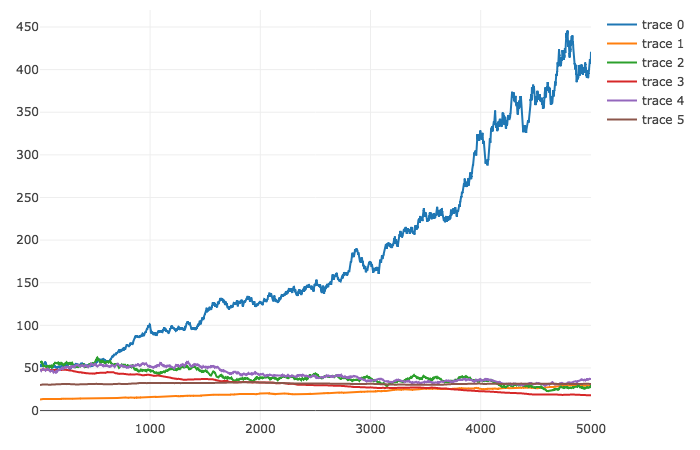
\includegraphics[scale=0.5]{images/synthetic_results/priceplot.png}
	\caption{Price Points}
	\label{figure-synthetic-prices}
\end{figure}


\subsubsection{SAE Network and Results}\label{results_synthetic_sae} 
\subsubsection{Predictive FFN Network and Results}

\paragraph{SAE Results}\mbox{}\\
\paragraph{Layer Size \& SGD Learning Rate Results}\mbox{}\\
\paragraph{OGD Learning Rate Results}\mbox{}\\
\paragraph{Prediction Plots}\mbox{}\\
\paragraph{CSCV Plots}\mbox{}\\
\subsection{Results for Real Data}

\newpage
\section{Conclusions}\label{Conclusion}



\newpage
\begin{thebibliography}{bibliography}

\bibitem{Albers}
Albers S. Online Algorithms: a survey. Mathematics Subject Classification (1991): 68W25, 
68W40. Available at: https://link.springer.com/content/pdf/10.1007%2Fs10107-003-0436-0.pdf

\bibitem{Aparicio}
Aparicio, Diego and Lopez de Prado, Marcos, How Hard Is It to Pick the Right Model? (December 2017). Available at SSRN: https://ssrn.com/abstract=3044740 or http://dx.doi.org/10.2139/ssrn.3044740

\bibitem{Arthur}
B. Arthur (1995) Complexity in Economics and Financial Markets, Complexity 1 (1), 20???25.

\bibitem{BailyPBO}
Bailey, David H. and Borwein, Jonathan and Lopez de Prado, Marcos and Zhu, Qiji Jim, The Probability of Backtest Overfitting (February 27, 2015). Journal of Computational Finance (Risk Journals), 2015, Forthcoming. Available at SSRN: https://ssrn.com/abstract=2326253 or http://dx.doi.org/10.2139/ssrn.2326253

\bibitem{BaileyBTL}
Bailey, David H. and Borwein, Jonathan and Lopez de Prado, Marcos and Zhu, Qiji Jim, Pseudo-Mathematics and Financial Charlatanism: The Effects of Backtest Overfitting on Out-of-Sample Performance (April 1, 2014). Notices of the American Mathematical Society, 61(5), May 2014, pp.458-471. Available at SSRN: https://ssrn.com/abstract=2308659 or http://dx.doi.org/10.2139/ssrn.2308659

\bibitem{BaileySharpe}
Bailey, David H. and Lopez de Prado, Marcos, The Deflated Sharpe Ratio: Correcting for Selection Bias, Backtest Overfitting and Non-Normality (July 31, 2014). Journal of Portfolio Management, 40 (5), pp. 94-107. 2014 (40th Anniversary Special Issue).. Available at SSRN: https://ssrn.com/abstract=2460551 or http://dx.doi.org/10.2139/ssrn.2460551

\bibitem{Bakiri}
G. Bakiri and T. G. Dietterich. Achieving high-accuracy text-to-speech with machine learning. In R. I. Damper, editor, Data Mining Techniques in Speech Synthesis. Chapman and Hall, New York, NY, 2002. 22

\bibitem{Bao}
Bao W, Yue J, Rao Y (2017) A deep learning framework for financial time series using stacked autoencoders and long-short term memory. PLoS ONE 12(7): e0180944. https://doi.org/10.1371/journal.pone.0180944

\bibitem{Bartlett}
Bartlett P., Hazan E. Adaptive Online Gradient Descent. Available at: http://papers.nips.cc/paper/3319-adaptive-online-gradient-descent.pdf

\bibitem{Bengio1}
Yoshua Bengio, Pascal Lamblin, Dan Popovici, and Hugo Larochelle. Greedy layer-wise training of deep networks. In Bernhard Scholkopf, John Platt, and Thomas Hoffman, editors, ¨ Advances in Neural Information Processing Systems 19 (NIPS’06), pages 153–160. MIT Press, 
2007. Available at: http://papers.nips.cc/paper/3048-greedy-layer-wise-training-of-deep-networks.pdf

\bibitem{Bengio2}
Bengio, Yoshua, and Samy Bengio. "Modeling high-dimensional discrete data with multi-layer neural networks." Advances in Neural Information Processing Systems. 2000.
Available at: http://papers.nips.cc/paper/1679-modeling-high-dimensional-discrete-data-with-multi-layer-neural-networks.pdf

\bibitem{Bengio3}
Bengio, Yoshua, Aaron Courville, and Pascal Vincent. "Representation learning: A review and new perspectives." IEEE transactions on pattern analysis and machine intelligence 35.8 (2013): 1798-1828.
Available at: https://ieeexplore.ieee.org/stamp/stamp.jsp?tp=\&arnumber=6472238\&tag=1

\bibitem{Bottou}
Bottou L., Le Cun Y. Large Scale Online Learning. Available at: http://papers.nips.cc/paper/2365-large-scale-online-learning.pdf

\bibitem{Bottou2}
Bottou, L. and Murata, N. (2002). Stochastic Approximations and Efficient Learning. In Arbib, M. A., editor, The Handbook of Brain Theory and Neural Networks, Second edition,. The MIT Press, Cambridge, 

\bibitem{Ciresan}
Cireşan, Dan Claudiu, et al. "Deep, big, simple neural nets for handwritten digit recognition." Neural computation 22.12 (2010): 3207-3220.
Available at: \url{https://www.mitpressjournals.org/doi/abs/10.1162/NECO_a_00052}

\bibitem{Chu}
Chu C., Time series segmentation: A sliding window approach. Information Sciences, Volume 85, Issues 1–3, July 1995, Pages 
147-173. Available at: \url{ttps://www.sciencedirect.com/science/article/pii/002002559500021G#!}

\bibitem{Chung}
 F. L. Chung, T. C. Fu, R. Luk, and V. Ng, “Flexible time series pattern matching based on perceptually important points,’’ in Proc. Int. Joint Conf. Artificial Intelligence Workshop  
 Learning from Temporal and Spatial Data in International Joint Conference on Artificial Intelligence (IJCAI'01), Seattle, Washington, USA, 4-10 August, 2001, p. 
 1-7. Available at: http://hdl.handle.net/10397/48578

\bibitem {Crutchfield}
J. P. Crutchfield, (2011), Between order and chaos, Nature Physics, Vol. 8, January 2012, 17-23

\bibitem{Dauphin}
Dauphin, Y. et al. Identifying and attacking the saddle point problem in high-dimensional non-convex optimization. In Proc. Advances in Neural Information Processing Systems 27 2933–2941 (2014)
Available at: http://papers.nips.cc/paper/5486-identifying-and-attacking-the-saddle-point-problem-in-high-dimensional-non-convex-optimization 

\bibitem{Devarakonda}
Aditya Devarakonda, Maxim Naumov \& Michael Garland. ADABATCH: ADAPTIVE BATCH SIZES FOR TRAINING
DEEP NEURAL NETWORKS. Available at: https://arxiv.org/pdf/1712.02029.pdf

\bibitem{Donoho}
David L. Donoho, High-Dimensional Data Analysis: The Curses and Blessings of 
Dimensionality (August 8, 2000). Available at: \url{http://citeseerx.ist.psu.edu/viewdoc/download?doi=10.1.1.329.3392&rep=rep1&type=pdf}

\bibitem{Duchi}
John Duchi, Elad Hazan and Yoram Singer. Adaptive Subgradient Methods for
Online Learning and Stochastic Optimization. Journal of Machine Learning Research 12 (2011) 
2121-2159. Available at: http://www.jmlr.org/papers/volume12/duchi11a/duchi11a.pdf

\bibitem{Erhan}
Erghan D., Bengio Y., Courville A, Manzagol P., Vincent P. Why Does Unsupervised Pre-training Help Deep 
Learning?, Journal of Machine Learning Research 11 (2010) 625-660 . Available 
at: http://www.jmlr.org/papers/volume11/erhan10a/erhan10a.pdf

\bibitem{Fama}
E.F. Fama, The behavior of stock-market prices, J. Bus., 1 (1965), pp. 34-105. 
Available at: https://doi.org/10.1086/294743

\bibitem{Fan1}
Jianqing Fan, Runze Li, 
Statistical Challenges with High Dimensionality: Feature Selection in Knowledge Discovery 
(7 Feb, 2006). Available at: https://arxiv.org/abs/math/0602133

\bibitem{Fan2}
Fan, J., \& Fan, Y. (2008). High Dimensional Classification Using Features Annealed Independence Rules. Annals of Statistics, 36(6), 2605–2637. http://doi.org/10.1214/07-AOS504

\bibitem {Ge}
Ge, Rong, et al. "Escaping from saddle points—online stochastic gradient for tensor decomposition." Conference on Learning Theory. 2015.
Available at: http://proceedings.mlr.press/v40/Ge15.pdf 

\bibitem{Goodfellow}
Goodfellow, Ian J., et al. "Maxout networks." arXiv preprint arXiv:1302.4389 (2013).
Available at: http://proceedings.mlr.press/v28/goodfellow13.pdf

\bibitem{Glorot}
Glorot, Xavier, and Yoshua Bengio. "Understanding the difficulty of training deep feedforward neural networks." Proceedings of the thirteenth international conference on artificial intelligence and statistics. 2010.
Available at: http://proceedings.mlr.press/v9/glorot10a/glorot10a.pdf

\bibitem{Glorot2}
Glorot, Xavier, Antoine Bordes, and Yoshua Bengio. "Deep sparse rectifier neural networks." Proceedings of the Fourteenth International Conference on Artificial Intelligence and Statistics. 2011.
Available at: http://proceedings.mlr.press/v15/glorot11a/glorot11a.pdf 

\bibitem{Griffioen} 
Griffioen, Gerwin A. W., Technical Analysis in Financial Markets (March 3, 2003).

\bibitem{Hansen}
Hansen, Peter Reinhard and Lunde, Asger and Nason, James M., The Model Confidence Set (March 18, 2010). Available at SSRN: https://ssrn.com/abstract=522382 or http://dx.doi.org/10.2139/ssrn.522382

\bibitem{Harvey}
Harvey, Campbell R. and Liu, Yan, Backtesting (July 28, 2015). Available at SSRN: https://ssrn.com/abstract=2345489 or http://dx.doi.org/10.2139/ssrn.2345489

\bibitem{Hawkins}
Hawkins, Douglas. (2004). The Problem of Overfitting. Journal of chemical information and computer sciences. 44. 1-12. 10.1021/ci0342472. 

\bibitem{Hinton1}
Geoffrey E. Hinton, Simon Osindero, and Yee Whye Teh. A fast learning algorithm for deep belief nets. Neural Computation, 18:1527–1554, 2006. 
Available at: https://www.mitpressjournals.org/doi/abs/10.1162/neco.2006.18.7.1527

\bibitem{Hinton2}
G. E. Hinton, R. R. Salakhutdinov, Reducing the Dimensionality of Data with Neural 
Networks. Science  28 Jul 2006: Vol. 313, Issue 5786, pp. 504-507 DOI: 
10.1126/science.1127647. Available at: http://science.sciencemag.org/content/313/5786/504/tab-pdf

\bibitem{Hinton3}
Geoffrey E. Hinton, Training Products of Experts by Minimizing Contrastive Divergence,Neural Computation
Volume 14 | Issue 8 | August 2002  p.1771-1800 . Available at: https://www.mitpressjournals.org/doi/pdf/10.1162/089976602760128018

\bibitem{Hinton4}
Hinton, Geoffrey E., et al. "Improving neural networks by preventing co-adaptation of feature detectors." arXiv preprint arXiv:1207.0580 (2012).
Available at: https://arxiv.org/pdf/1207.0580.pdf

\bibitem{HLZ}
Campbell R. Harvey \& Yan Liu \& Heqing Zhu, 2016. "… and the Cross-Section of Expected Returns," Review of Financial Studies, vol 29(1), pages 5-68.

\bibitem{Hochreiter}
Sepp Hochreiter,  Jürgen Schmidhuber. Long Short-Term Memory. Neural Computation Volume 9 | Issue 8 | November 15, 1997  
p.1735-1780. Available at https://www.mitpressjournals.org/doi/abs/10.1162/neco.1997.9.8.1735.

\bibitem {Hornik}
K. Hornik, Multilayer feed-forward networks are universal approximators, Neural Networks, vol 2, 1989

\bibitem{Hsu}
Hsu D. Time Series Compression Based on Adaptive Piecewise
Recurrent Autoencoder (17 August 2017). Available at: https://arxiv.org/pdf/1707.07961.pdf

\bibitem{Ivakhnenko}
Ivakhnenko, A. G. (1971). Polynomial theory of complex systems. IEEE Transactions
on Systems, Man and Cybernetics, (4), 364–378. Available at: https://ieeexplore.ieee.org/document/4308320/

\bibitem{ImageNet}
Krizhevsky, Alex, Ilya Sutskever, and Geoffrey E. Hinton. "Imagenet classification with deep convolutional neural networks." Advances in neural information processing systems. 2012.
Available at: http://papers.nips.cc/paper/4824-imagenet-classification-with-deep-convolutional-neural-networks

\bibitem{Ioannidis} 
Ioannidis JPA (2005) Why Most Published Research Findings Are False. PLoS Med 2(8): e124. https://doi.org/10.1371/journal.pmed.0020124

\bibitem {Johnson}
N. Johnson, G. Zhao, E. Hunsader, H. Qi, N. Johnson, J. Meng \& Brian Tivnan (2013). Abrupt rise of new machine ecology beyond human response time. Sceintific Reports 3(2627). DOI: 10.1038/srep02627

\bibitem{Kahn}
Kahn, Michael N. . Technical Analysis Plain and Simple: Charting the Markets in Your Language, Financial Times Press, Upper Saddle River, New Jersey, p. 9. ISBN 0-13-134597-4.(2006)

\bibitem{Knerr}
Stefan Knerr, Handwritten Digit Recognition by Neural Networks with Single-Layer 
Training. 962 IEEE TRANSACTIONS ON NEURAL NETWORKS, VOL. 3, NO. 6, NOVEMBER 
1992. Available at: \url{https://ieeexplore.ieee.org/stamp/stamp.jsp?tp=&arnumber=165597 }


\bibitem{Langford}
John Langford, Lihong Li and Tong Zhang. Sparse Online Learning via Truncated 
Gradient. Journal of Machine Learning Research 10 (2009) 777-801 Submitted 6/08; Revised 11/08; Published 
3/09. Available at: http://www.jmlr.org/papers/volume10/langford09a/langford09a.pdf 

\bibitem{Langkvist}
Martin Längkvist, Lars Karlsson,  Amy Loutfi, A review of unsupervised feature learning and deep learning for time-series 
modeling, Applied Autonomous Sensor Systems, School of Science and Technology, Örebro University, SE-701 82 Örebro, 
Sweden. Available at: \url{https://www.sciencedirect.com/science/article/pii/S0167865514000221#bi005}

\bibitem{LeCun}
LeCun Y., Bottou L, Orr G, Muller K. Efficient Backprop. Available at: http://yann.lecun.com/exdb/publis/pdf/lecun-98b.pdf

\bibitem{LeCun2}
LeCun, Y. (1988). A theoretical framework for back-propagation. In D. Touretzky,
G. Hinton, \& T. Sejnowski (Eds.), Proceedings of the 1988 connectionist models summer school (pp. 21–28).
\url{Available at: https://www.researchgate.net/profile/Yann_Lecun/publication/2360531_A_Theoretical_Framework_for_Back-Propagation/links/0deec519dfa297eac1000000/A-Theoretical-Framework-for-Back-Propagation.pdf}

\bibitem{LeCun3}
LeCun, Y., Boser, B., Denker, J. S., Henderson, D., Howard, R. E., Hubbard, W., et al.
(1989). Back-propagation applied to handwritten zip code recognition. Neural
Computation, 1(4), 541–551. Available at: http://papers.nips.cc/paper/293-handwritten-digit-recognition-with-a-back-propagation-network.pdf

\bibitem{LeCun4}
Yann LeCun, Yoshua Bengio \& Geoffrey Hinton. Deep learning, Nature volume 521, pages 436–444 (28 May 
2015). Available at: https://www.nature.com/articles/nature14539

\bibitem{LeRoux}
Le Roux, Nicolas, and Yoshua Bengio. "Representational power of restricted Boltzmann machines and deep belief networks." Neural computation 20.6 (2008): 1631-1649.
Available at: http://www.iro.umontreal.ca/~lisa/publications2/index.php/attachments/single/22

\bibitem{Liu}
Liu X., Lin Z., Wang H. Novel Online Methods for Time Series Segmentation.  IEEE TRANSACTIONS ON KNOWLEDGE AND DATA ENGINEERING, VOL. 20, NO. 12, DECEMBER 
2008. Available at: \url{https://ieeexplore.ieee.org/stamp/stamp.jsp?arnumber=4445667&tag=1}

\bibitem{Lo}
Lo, Andrew W., The Statistics of Sharpe Ratios. Financial Analysts Journal, Vol. 58, No. 4, July/August 2002. Available at SSRN: https://ssrn.com/abstract=377260

\bibitem{Lv}
Yisheng Lv, Yanjie Duan, Wenwen Kang, Zhengxi Li, and Fei-Yue Wang. Traffic Flow Prediction With Big Data:
A Deep Learning Approach. IEEE TRANSACTIONS ON INTELLIGENT TRANSPORTATION SYSTEMS, VOL. 16, NO. 2, APRIL 
2015. Available at: \url{https://ieeexplore.ieee.org/stamp/stamp.jsp?tp=&arnumber=6894591&tag=1}

\bibitem{Mahajan}
Mahajan D., Keerthi S., Sundararajan S., Bottou L. A Parallel SGD method with Strong 
Convergence. Available at: https://arxiv.org/pdf/1311.0636.pdf

\bibitem{McLean}
McLean, R. David and Pontiff, Jeffrey, Does Academic Research Destroy Stock Return Predictability? (January 7, 2015). Journal of Finance, Forthcoming. Available at SSRN: https://ssrn.com/abstract=2156623 or http://dx.doi.org/10.2139/ssrn.2156623

\bibitem{Minksy}
M Minsky, SA Papert, L Bottou (1988). Perceptrons: An introduction to computational  geometry. Available at: \url{https://books.google.co.za/books?hl=en&lr=&id=PLQ5DwAAQBAJ&oi=fnd&pg=PR5&dq=Minsky+Papert+1969+%E2%80%94+Perceptrons&ots=zyEDwMvmXX&sig=aVXF7DBJKAOxW066S4UCyzhNARw#v=onepage&q=Minsky%20Papert%201969%20%E2%80%94%20Perceptrons&f=false}

\bibitem{Murphy}
Murphy, John J. Technical analysis of the financial markets: A comprehensive guide to trading methods and applications. Penguin, 1999.

\bibitem{Pascanu}
Pascanu, Razvan, Tomas Mikolov, and Yoshua Bengio. "On the difficulty of training recurrent neural networks." International Conference on Machine Learning. 2013.
Available at: http://proceedings.mlr.press/v28/pascanu13.pdf

\bibitem{Prado}
Lopez de Prado, Marcos, The Future of Empirical Finance (May 31, 2015). Journal of Portfolio Management, 41(4). Summer 2015. Forthcoming.. Available at SSRN: https://ssrn.com/abstract=2609734 or http://dx.doi.org/10.2139/ssrn.2609734

\bibitem{Povey}
Povey D., Zhang X., Khudanpur S. Parallel training of Deep Neural Networks with Natural Gradient and Parameter Averaging. Available at: \url{http://citeseerx.ist.psu.edu/viewdoc/download?doi=10.1.1.745.6995&rep=rep1&type=pdf}

\bibitem{Ranzato1}
Marc’Aurelio Ranzato, Christopher Poultney, Sumit Chopra, and Yann LeCun. Efficient learning of sparse representations with an energy-based model. In B. Scholkopf, J. Platt, and T. Hoffman, ¨ editors, Advances in Neural Information Processing Systems 19 (NIPS’06), pages 1137–1144. MIT Press, 
2007. Aavilable at: http://papers.nips.cc/paper/3112-efficient-learning-of-sparse-representations-with-an-energy-based-model.pdf

\bibitem{Rumelhart}
Rumelhart, D. E., Hinton, G. E., \& Williams, R. J. (1986). Learning internal representations by error propagation. In D. E. Rumelhart, \& J. L. McClelland (Eds.), Parallel distributed processing, vol. 1 (pp. 318–362). MIT Press.

\bibitem{Schaefer}
Robert L. Schaefer (2012) Subset Selection in Regression, Technometrics, 34:2, 229, DOI: 10.1080/00401706.1992.10484917
  
 \bibitem{Schmidhuber}
J Schmidhuber (2015). Deep learning in neural networks: An overview. Neural Networks Volume 61, January 2015, Pages 
85-117. Available at https://www.sciencedirect.com/science/article/pii/S0893608014002135. 
  
\bibitem{Schorfheide}
Schorfheide, Frank, and Kenneth I. Wolpin. 2012. "On the Use of Holdout Samples for Model Selection." American Economic Review, 102 (3): 477-81.

\bibitem {Schwager}
Jack D. Schwager. Getting Started in Technical Analysis, Page 2 (1999)


\bibitem{Sermanet}
Sermanet, Pierre, et al. "Pedestrian detection with unsupervised multi-stage feature learning." Computer Vision and Pattern Recognition (CVPR), 2013 IEEE Conference on. IEEE, 2013.
Available at: https://arxiv.org/abs/1212.0142

\bibitem{Shalev}
Shai Shalev-Shwartz, Yoram Singer, and Nathan Srebro. Pegasos: Primal Estimated sub-GrAdient SOlver for SVM. In Proceedings of the Twenty-Fourth International Conference on Machine Learning (ICML-07), 2007.

\bibitem{Siegelmann}
Siegelmann, H. (1992). Theoretical foundations of recurrent neural networks (Ph.D. thesis), New Brunswick Rutgers, The State of New Jersey: Rutgers. Available at: \url{http://citeseerx.ist.psu.edu/viewdoc/download?doi=10.1.1.38.920&rep=rep1&type=pdf}

\bibitem {Skabar}
 Skabar, Cloete, Networks, Financial Trading and the Efficient Markets Hypothesis (http://crpit.com/confpapers/CRPITV4Skabar.pdf)

\bibitem{Takeuchi}
Takeuchi L, Lee Y. Applying Deep Learning to Enhance Momentum Trading Strategies in 
Stocks. Technical Report, 2013. Available at: http://www.smallake.kr/wp-content/uploads/2017/04/TakeuchiLee-ApplyingDeepLearningToEnhanceMomentumTradingStrategiesInStocks.pdf

\bibitem{Troiano}
Troiano L., Mejuto E., Kriplani P.On Feature Reduction using Deep Learning
for Trend Prediction in Finance (11 Apr 2017).  Available at: 
https://arxiv.org/abs/1704.03205.

\bibitem{Tseng}
Tseng P., AN INCREMENTAL GRADIENT(-PROJECTION) METHOD
WITH MOMENTUM TERM AND ADAPTIVE STEPSIZE RULE. SIAM J. OPTIM.  Vol. 8, No. 2, pp. 506–531, May 
1998. Available at: https://pdfs.semanticscholar.org/1a29/6a1577478654a54a9f801f93f71b7d853c53.pdf

\bibitem{Vincent}
Vincent P., Larochell H., Lajoie I., Bengio Y., Manzagol P., Stacked Denoising Autoencoders: Learning Useful Representations in
a Deep Network with a Local Denoising Criterion. Journal of Machine Learning Research 11 (2010) 
3371-3408. Available at: http://www.jmlr.org/papers/volume11/vincent10a/vincent10a.pdf

\bibitem{Wan}
Wan Y., Gong X., Si Y. Effect of segmentation on financial time series pattern 
matching. Applied Soft Computing Volume 38, January 2016, Pages 346-359. 
Available at: https://www.sciencedirect.com/science/article/pii/S1568494615006341

\bibitem {Wang}
Linnan Wang,  Yi Yang, Renqiang Min, Srimat Chakradhar. Accelerating deep neural network training with 
inconsistent stochastic gradient descent. Neural Networks
Volume 93, September 2017, Pages 219-229. Available at: https://www.sciencedirect.com/science/article/pii/S0893608017301399

\bibitem{Wang2}
Wang, Sida, and Christopher Manning. "Fast dropout training." international conference on machine learning. 2013.
Available at: http://proceedings.mlr.press/v28/wang13a.pdf

\bibitem{WaveNet}
Van Den Oord, Aaron, et al. "Wavenet: A generative model for raw audio." arXiv preprint arXiv:1609.03499 (2016).
Available at: https://arxiv.org/abs/1609.03499

\bibitem{Weiss}
Weiss, S. M, \& Kulikowski, C. A. (1991). Computer systems that learn : classification and prediction methods from statistics, neural nets, machine learning, and expert systems. San Mateo (Calif.): Kaufmann.

\bibitem{Werbos}
Werbos, P. J. (1974). Beyond regression: new tools for prediction and analysis in the behavioral sciences (Ph.D. thesis), Harvard 
University. Available at: \url{https://www.researchgate.net/publication/244947191_1974_Beyond_regression_New_tools_for_predicting_and_analysis_in_the_behavioral_sciences}

\bibitem{Werbos2}
Paul J. Werbos. Applications of advances in nonlinear sensitivity analysis. 
System Modeling and Optimization pp 762-770. Available at: https://link.springer.com/chapter/10.1007/BFb0006203

\bibitem{Wu}
Wu, Huaiqin. "Global stability analysis of a general class of discontinuous neural networks with linear growth activation functions." Information Sciences 179.19 (2009): 3432-3441.
Available at: \url{https://ac.els-cdn.com/S0020025509002539/1-s2.0-S0020025509002539-main.pdf?_tid=fc9d5d20-c0fe-4107-947c-6a4d9e472aab&acdnat=1526319168_bc401e01e4ab496b50b8d568dcafb0b3}

\bibitem{Yin}
Yin J., Si Y., Gong Z. Financial Time Series Segmentation Based On Turning 
Points. Proceedings of 2011 International Conference on System Science and Engineering, Macau, China - June 
2011. Available at: \url{https://ieeexplore.ieee.org/stamp/stamp.jsp?tp=&arnumber=5961935}

\bibitem{Zeiler}
Zeiler M. ADADELTA: An Adaptive Learning Rate Method. Available at: https://arxiv.org/abs/1212.5701

\bibitem{Zinkevich}
Zinkevich M, Weimer M, Smola A, Li L. Parallelized Stochastic Gradient Descent. 
Available at: 
http://papers.nips.cc/paper/4006-parallelized-stochastic-gradient-descent.pdf

\bibitem{Zhao}
Zhao Y., Li J., Yu L. A deep learning ensemble approach for crude oil price 
forecasting.  Available at: https://doi.org/10.1016/j.eneco.2017.05.023

\bibitem{Zhang}
Tong Zhang. Solving large scale linear prediction problems using stochastic gradient descent algorithms. In Proceedings of the Twenty-First International Conference on Machine Learning (ICML-04), pages 919–926, 2004

\bibitem{Zhou}
Zhou B., Hu J. A Dynamic Pattern Recognition Approach Based on Neural Network for Stock Time-Series. 2009 World Congress on Nature \& Biologically Inspired Computing (NaBIC 
2009). Available at:\url{ https://ieeexplore.ieee.org/stamp/stamp.jsp?tp=&arnumber=5393674}

\end{thebibliography}
\end {document}





